% Version 5.0, 2 January 2020

% This tex file can be compiled with
% tectonic templateV5.tex
% https://tectonic-typesetting.github.io
%
% Or simply with the Overleaf latexmkrc configuration: (included in the repo)
% https://www.overleaf.com/learn/how-to/How_does_Overleaf_compile_my_project%3F
%
% A latexindent.yml config file is also included for easier and more consistent
% formatting.

% %%%%%%%%%%%%%%%%%%%%%%%%%%%%%%%%%%%%%%%%%%%%%%%%%%%%%%%%%%%%%%%%%%%%%%%%%%%%%%%%%%%%%%
% TemplateV5.tex -- LaTeX-based template for submissions to the American Meteorological
% Society
% %%%%%%%%%%%%%%%%%%%%%%%%%%%%%%%%%%%%%%%%%%%%%%%%%%%%%%%%%%%%%%%%%%%%%%%%%%%%%%%%%%%%%%
% PREAMBLE
% %%%%%%%%%%%%%%%%%%%%%%%%%%%%%%%%%%%%%%%%%%%%%%%%%%%%%%%%%%%%%%%%%%%%%%%%%%%%%%%%%%%%%%

% Start with one of the following: DOUBLE-SPACED VERSION FOR SUBMISSION TO THE AMS
\documentclass{ametsocV5}

% TWO-COLUMN JOURNAL PAGE LAYOUT---FOR AUTHOR USE ONLY
% \documentclass[twocol]{ametsocV5}

% Enter packages here. If too many math alphabets are used, remove unnecessary packages
% or define hmmax and bmmax as necessary.
%\newcommand{\hmmax}{0}
%\newcommand{\bmmax}{0}
\usepackage{amsmath,amsfonts,amssymb,bm}
\usepackage{mathptmx}% {times}
\usepackage{newtxtext}
\usepackage{newtxmath}
\usepackage[version=4]{mhchem}
\usepackage[acronym]{glossaries}
\usepackage{cleveref}
\usepackage[separate-uncertainty=true]{siunitx}
\usepackage{listings}
% \usepackage{hyperref}

\makeglossaries{}
\newacronym{agcm}{AGCM}{Atmosphere General Circulation Model}
\newacronym{aodm}{AODVISstdn}{``stratospheric aerosol optical depth 550 nm day night''}
\newacronym{aod}{AOD}{(stratospheric) aerosol optical depth}
\newacronym{aogcm}{AOGCM}{Atmosphere-Ocean General Circulation Model}
\newacronym{c2wmp}{C2W\(-\)}{CESM2(WACCM6) intermediate strength}
\newacronym{c2wm}{C2W\(\downarrow\)}{CESM2(WACCM6) small strength}
\newacronym{c2wsn}{C2WN\(\uparrow\)}{CESM2(WACCM6) large strength, high northern latitude}
\newacronym{c2ws}{C2W\(\uparrow\)}{CESM2(WACCM6) large strength}
\newacronym{c2w}{C2W}{CESM2(WACCM6) tropical}
\newacronym{cam5}{CAM5}{Community Atmosphere Model Version 5}
\newacronym{cam6}{CAM6}{Community Atmosphere Model Version 6}
\newacronym{cesm1}{CESM1}{Community Earth System Model Version 1}
\newacronym{cesm2}{CESM2}{Community Earth System Model Version 2}
\newacronym{cesm}{CESM}{Community Earth System Model}
\newacronym{cice}{CICE5}{CICE Version 5.1.2}
\newacronym{cime}{CIME}{Common Infrastructure for Modelling the Earth}
\newacronym{cism}{CISM2}{Community Ice Sheet Model Version 2.1}
\newacronym{clm}{CLM5}{Community Land Model Version 5}
\newacronym{ecs}{ECS}{equilibrium climate sensitivity}
\newacronym{erf}{ERF}{effective radiative forcing}
\newabbreviation{ob16}{OB16}{\citet{ottobliesner2016}}
\newacronym{esm}{ESM}{Earth System Model}
\newacronym{flnt}{FLNT}{``net longwave flux at the top of the model''}
\newacronym{fpp}{FPP}{Filtered Poisson Process}
\newacronym{fsnt}{FSNT}{``net solar flux at the top of the model''}
\newacronym{fsst}{\texttt{fSST1850}}{fixed sea-surface temperature}
\newacronym{irf}{IRF}{instantaneous radiative forcing}
\newacronym{lwcf}{LWCF}{``long wave cloud forcing''}
\newacronym{lw}{LW}{long wave}
\newacronym{mam3}{MAM3}{three mode version of the Modal Aerosol Module}
\newacronym{mam}{MAM}{Modal Aerosol Module}
\newacronym{marbl}{MARBL}{MARine Biogeochemistry Library}
\newacronym{ma}{MA}{middle atmosphere}
\newacronym{mosart}{MOSART}{MOdel for Scale Adaptive River Transport}
\newabbreviation{j05}{J05}{\citet{jones2005}}
\newabbreviation{g16}{G16}{\citet{gregory2016}}
\newabbreviation{m20}{M20}{\citet{marshall2020dataset}}
\newabbreviation{t10}{T10}{\citet{timmreck2010}}
\newabbreviation{n15}{N15}{\citet{niemeier2015}}
\newacronym{pop}{POP2}{Parallel Ocean Program Version 2}
\newacronym{qbo}{QBO}{quasi-biennial oscillation}
\newacronym{rf}{RF}{(effective) radiative forcing}
\newacronym{swcf}{SWCF}{``short wave cloud forcing''}
\newacronym{sw}{SW}{short wave}
\newacronym{tcrp}{TCRP}{transient climate response parameter}
\newacronym{toa}{TOA}{top-of-the-atmosphere}
\newacronym{trefht}{TREFHT}{``reference height temperature''}
\newacronym{waccm}{WACCM6}{Whole Atmosphere Community Climate Model Version 6}
\newacronym{ww3}{WW3}{Wave Watch Version 3}
\newacronym{ytt}{YTT}{Young Toba Tuff}


% Create some custom commands
\newcommand{\iso}[1][i]{{#1}njected \ce{SO2}}

% %%%%%%%%%%%%%%%%%%%%%%%%%%%%%%%%%%%%%%%%%%%%%%%%%%%%%%%%%%%%%%%%%%%%%%%%%%%%%%%%%%%%%%

% To be entered by author:
% May use \\ to break lines in title:
\title{
  Parameter Scan: Volcanic influence on climate across multiple magnitudes of injected
  \ce{SO2}
}

% Enter authors' names, as you see in this example: Use \correspondingauthor{} and
% \thanks{Current Affiliation:...} immediately following the appropriate author. Note
% that the \correspondingauthor{} command is NECESSARY. The \thanks{} commands are
% OPTIONAL.

\authors{
  Eirik Rolland Enger\correspondingauthor{Eirik Rolland Enger, eirik.r.enger@uit.no}
}

% Follow this form: \affiliation{American Meteorological Society, Boston, Massachusetts}
\affiliation{UiT The Arctic University of Norway, Tromsø, Norway}

% \affiliation{}

% If appropriate, add additional authors, different affiliations:
\extraauthor{Audun Theodorsen}
\extraaffil{UiT The Arctic University of Norway, Tromsø, Norway}
\extraauthor{Rune Graversen}
\extraaffil{UiT The Arctic University of Norway, Tromsø, Norway}
\extraauthor{Martin Rypdal}
\extraaffil{UiT The Arctic University of Norway, Tromsø, Norway}
\extraauthor{Maria Rugenstein}
\extraaffil{Colorado State University, Fort Collins, Colorado}

% %%%%%%%%%%%%%%%%%%%%%%%%%%%%%%%%%%%%%%%%%%%%%%%%%%%%%%%%%%%%%%%%%%%%%%%%%%%%%%%%%%%%%%
% ABSTRACT
%
% Enter your abstract here. Abstracts should not exceed 250 words in length!

\abstract{
  Volcanoes affect Earth's climate. What happens when the climate is forced with
  volcanoes of different size and injected at different heights? Should we expect to see
  the same climate response for the same volcanoes in a different, warmer climate?
}

\begin{document}

% Necessary!
\maketitle

% %%%%%%%%%%%%%%%%%%%%%%%%%%%%%%%%%%%%%%%%%%%%%%%%%%%%%%%%%%%%%%%%%%%%%%%%%%%%%%%%%%%%%%
% SIGNIFICANCE STATEMENT/CAPSULE SUMMARY
% %%%%%%%%%%%%%%%%%%%%%%%%%%%%%%%%%%%%%%%%%%%%%%%%%%%%%%%%%%%%%%%%%%%%%%%%%%%%%%%%%%%%%%
%
% If you are including an optional significance statement for a journal article or a
% required capsule summary for BAMS (see
% www.ametsoc.org/ams/index.cfm/publications/authors/journal-and-bams-authors/formatting-and-manuscript-components
% for details), please apply the necessary command as shown below:
%
% \statement
% Significance statement here.
%
% \capsule
% Capsule summary here.

% %%%%%%%%%%%%%%%%%%%%%%%%%%%%%%%%%%%%%%%%%%%%%%%%%%%%%%%%%%%%%%%%%%%%%%%%%%%%%%%%%%%%%%
% MAIN BODY OF PAPER
% %%%%%%%%%%%%%%%%%%%%%%%%%%%%%%%%%%%%%%%%%%%%%%%%%%%%%%%%%%%%%%%%%%%%%%%%%%%%%%%%%%%%%%

% In all cases, if there is only one entry of this type within the higher level heading,
% use the star form:
%
% \section{Section title}
% \subsection*{subsection}
% text...
% \section{Section title}
%
% vs
%
% \section{Section title}
% \subsection{subsection one}
% text...
% \subsection{subsection two}
% \subsubsection{First tertiary heading}
% \paragraph{First quaternary heading}
% \section{Section title}

% NOTE: what to include in the paper, key questions.
% The paper should provide insight about what might happen if a large volcano erupted
% (order of magnitude or more than Mount Pinatubo). How does the atmosphere react, for
% example in the aerosol dynamics? (QBO, SO2/AOD/RF relationship.) It should also be
% about how volcanic simulations compare in magnitude and if there is time for more
% simulations, how model complexity (dynamic ocean against slab ocean) affect things.
% - How far does the linear relation between AOD and RF go? What phases does the
%   aerosols go though? (Perhaps the most promising avenue.)
% - How much does it matter how high in the atmosphere the initial SO2 is injected?
%   (Already is some literature on this, suggesting it is not much. Also some on
%   latitude dependence, which has a bigger influence.)
% - How does the climate response change based on the state of the climate: what if we
%   run a CO2 doubling or quadrupling simulation until close to equilibrium, and let the
%   volcanoes erupt then? (Lack the doubling scenario, and setting it up has resulted in
%   strange output that must be resolved. Could take a while.)

\section{Introduction and Motivation}

\paragraph*{Why volcanoes have been given attention}

During much of the past few thousand years, the Holocene, the natural climate
variability on Earth have been mostly forced by volcanic eruptions \citep{sigl2022}.
Despite the strong influence volcanic eruptions have on climate variability, in
particular up to the current strong anthropogenic forcing of the climate, few climate
model experiments have included volcanic forcing estimates when simulating climate
evolution \citep{sigl2022}, implying an incorrect positive forcing \citep{gregory2016}.
Thus, even though understanding how volcanic eruptions force the climate has been given
much attention, many questions still remain unanswered
\citep[e.g.,][]{robock2000,zanchettin2019,marshall2022}.

% Section on similarities between CO2 and volcanic forcing. (feedback params
% references). Richardson is doing something that looks very similar to Gunther 2022.
% Mention that as well? (Similarity bw 0.5CO2 and volcanoes.)

\paragraph*{On similarities bw.\ \ce{CO2} and volcanoes (\acrshort{ecs})}

One avenue that have been given much attention is how forcing from volcanoes or
volcano-like forcings compare to the forcing that is due to increased \ce{CO2} levels.
\citet{boer2007,marvel2016,merlis2014,ollila2016,richardson2019,salvi2022,wigley2005}
all look at the link or lack thereof between volcanic forcing and the climate
sensitivity to a doubling of \ce{CO2}, a much used metric for describing the severity of
global warming \citep{marvel2016}. This is motivated by the large uncertainty in
estimates of the sensitivity of the real climate system, and inferring climate
sensitivity from for example volcanoes have been used as an attempt to constrain the
sensitivity \citep{boer2007}. Among these, some have been running simulations of the
1991 Mt.\ Pinatubo eruption \citep{merlis2014,ollila2016} or historical volcano or
volcano-like forcings \citep{boer2007,marvel2016,wigley2005}, while some look at aerosol
forcing in general \citep{richardson2019,salvi2022}. While many of the earlier studies
often assume \acrshort{ecs} can be inferred from volcanoes \citep{wigley2005} or suggest
that it might be possible \citep{bender2010}, as long as you constrain it with
\acrfull{erf} and not \acrfull{irf} \citep{richardson2019}, other studies suggest this
is either not possible and that the sensitivity to volcanic forcing and \ce{CO2}
doubling are different or that the precision at which climate simulations are run must
be much higher \citep{douglass2006,boer2007,salvi2022}. However, even though
\acrshort{erf} is a more suited indicator of the temperature response to a forcing than
\acrshort{irf} \citep{marvel2016,richardson2019}, more recent studies conclude that
\acrshort{ecs} cannot be constrained from volcanoes \citep{pauling2023}.

% TODO: write section on aerosol evolution in the atmosphere (Robock 2000, Pitari 2016).
% Something related to loop in figures.

\paragraph*{On aerosol evolution and atm.\ dynamics}

Even though \ce{H2O}, \ce{N2} and \ce{CO2} are the most abundant gases emitted by
volcanoes \citep{robock2000}, sulphur species like \ce{SO2} are the most influential due
to the already large concentrations of the former gases in the atmosphere. From \ce{SO2}
comes \ce{H2SO4} due to reactions with \ce{OH} and \ce{H2O} \citep{robock2000}. Sulphate
acid, \ce{H2SO4}, produce the largest effect on the radiative forcing, and since their
formation from \ce{SO2} is happening over weeks \citep{robock2000}, the peak radiative
forcing from the eruption has a slight delay from the eruption time. The duration of
time that the \ce{H2SO4} aerosols stay in the atmosphere depends on several factors,
including the phase of the \acrshort{qbo} \citep{pitari2016b}, the season of the year
(most notably to which hemisphere aerosols are transported)
\citep{toohey2011,toohey2019}, latitude \citep{marshall2019,toohey2019}, volcanic plume
height \citep{marshall2019} and their size \citep{marshall2019}. In the case of tropical
eruptions, aerosols are typically transported poleward in the stratosphere and back to
mid-latitude troposphere within one to two years \citep{robock2000}.

% Section on RF to AOD ratio

\paragraph*{On the comparison bw.\ \acrshort{rf} and \acrshort{aod}}

Previous studies on both Mt. Pinatubo alone \citep{mills2017,hansen2005} and volcanoes
in the instrumental era \citep{gregory2016} have been used to estimate the relationship
between the energy imbalance caused by volcanic eruptions and \acrshort{aod}.
\citet{myhre2013} use a formula for \acrshort{rf} that scales \acrshort{aod} by
\(\SI{-25}{\watt\metre^{-2}\mathrm{SAOD}^{-1}}\) while values down to
\(\SI{-19.0(5)}{\watt\metre^{-2}\mathrm{SAOD}^{-1}}\) \citep{gregory2016} and
\(\SI{-18.3(10)}{\watt\metre^{-2}\mathrm{SAOD}^{-1}}\) \citep{mills2017} have been
reported more recently. Simulations done with synthetic volcanoes have also been used,
and in \citet{marshall2020} they simulate a total of \(82\) volcanic eruptions with
varying injection height and latitude, ranging from \(10\) to \(\SI{100}{\tera\gram}\)
of \iso{}. They obtain a scaling factor of
\(\SI{-20.5(2)}{\watt\metre^{-2}\mathrm{SAOD}^{-1}}\) \citep{marshall2020}.

A similar simulation setup, albeit with significant differences, was done by
\citet{niemeier2015}, where \(14\) different levels of injected sulphur ranging between
\(\SI{1}{\tera\gram(\ce{S})\mathrm{yr}^{-1}}\)
(\(\SI{2}{\tera\gram(\ce{SO2})\mathrm{yr}^{-1}}\)) and
\(\SI{100}{\tera\gram(\ce{S})\mathrm{yr}^{-1}}\)
(\(\SI{200}{\tera\gram(\ce{SO2})\mathrm{yr}^{-1}}\)) was simulated. These were
geoengineering simulations where sulphur would be continually injected, and the
simulations run until the sulphur level was in a steady state. From this, they found
that the radiative forcing to injecting rate ratio would follow an exponential and
converge to a value of \(\SI{-65}{\watt\metre^{-2}}\). While the results from the
super-volcano simulation by \citet{jones2005} indicate a much less steep gradient than
the \(-18.3\) to \(-25\) found in more recent literature, the peak radiative forcing
obtained in the super-volcano simulation was \(\SI{-60}{\watt\metre^{-2}}\), which may
suggest the \citet{niemeier2015} results to be transferable to a volcanic eruption
simulation scenario.

\paragraph*{Aerosol optical depth vs.\ radiative forcing}

The aerosol evolution and lifetime in the stratosphere strongly influence the radiative
forcing resulting from the aerosols and the \acrshort{aod}, but not always in the same
way. \citet{marshall2020} present results showing higher efficacies in years 2 and 3
after an eruption, compared to year 1, explaining that this is due to the aerosols being
concentrated more spatially in the first year and more spread out in later years. This
has the effect of increasing the albedo per global mean \acrshort{aod} which in turn
increases the \acrshort{rf} per \acrshort{aod} \citep{marshall2020}. (Also,
\acrshort{saod} to \acrshort{rf} depend on insulation, cloudiness and surface albedo
among others, which vary across eruptions \citep{marshall2021,andersson2015}.)

% \citet{marshall2022} mention (in the graphic in their figure 1) that the \emph{role of
%   initial conditions} is a key outstanding question, especially if the \ce{CO2}
% doubling simulations work out, this could be a contribution to that.
% Also, when aerosols grow, they scatter radiation less efficiently and also fall down
% faster, so the temperature response should be comparatively weaker for increasing
% eruption magnitude (or the volcanic aerosols are less efficient). \emph{Clustering} and
% long term effects are mentioned in its own section (Multi-decadal impacts) along with
% the \emph{dependence of the current climate state}.

% \citet{marshall2019} does many similar things to what I have done, but do not focus on
% seasonal variability. This is however mentioned as one other direction to dig into, but
% is somewhat covered by \citet{marshall2020}. Assumes that there is an $e$-folding time,
% but notes that it does change, so they calculate an average time over a small range
% (from a month after the peak until reaching ten percent of the peak). They further note
% that the $e$-folding time is dependent on latitude mostly, but also on injected
% \ce{SO2}. Their eruptions all occur in July, but with the equivalent winter (January)
% eruptions covered by \citet{marshall2020}.

% In \citet{marshall2020}, they take the reconstructed \acrshort{saod} from
% \citet{toohey2017}, convert it to radiative forcing based on their conversions, and plot
% the corresponding temperature time series from each radiative forcing using a simple
% climate model. \emph{So, can we use this with the \acrfull{fpp} framework? (Noisy data?
%   Check this.)}
% TODO: check the data if it can be used for FPP.

% Perhaps focus on why there seems to be a loop in the \acrshort{aod} against
% \acrshort{rf} plots. Can also compare February-August means with May-November means.
% (\citet{marshall2021} discuss Tambora, but mention that it erupted in April, while their
% data consist of January and July eruptions.)

\paragraph*{Motivation}

From \citet{pauling2023}: what aspect of the climate system control the response to
volcanic eruptions?

From \citet{marshall2022}: However, uncertainties remain regarding the role of internal
variability and the dependence on the current climate state. Also \citet{aubry2022} give
a review on this very topic. They emphasise the urgency to accelerate research on
climate-volcano impacts (a niche topic to date).

\section{Method}

\subsection{Output variables}

% TODO: describe ERF vs IRF, and what is used here (for example Marshall 20??,
% Richardson 2019, Marvel 2016)

Radiative forcing is calculated as the combined (\acrshort{sw} and \acrshort{lw})
all-sky \acrshort{toa} energy imbalance, where the \acrshort{cesm2} provide the output
variables \acrfull{fsnt} and \acrfull{flnt}. We thus get that \(\mathrm{RF_*}=
\mathrm{FSNT} - \mathrm{FLNT}\) and taking the difference between volcanic simulations
and a control simulation gives the final estimate of \acrshort{rf}
(\(\mathrm{RF}=\mathrm{RF_{VOLC}}-\mathrm{RF_{CONTROL}}\)) \citep{marshall2020}. The
\acrshort{aod} is obtained from the output variable \acrfull{aodm}, while global
temperature is saved by \acrshort{cesm2} to the variable \acrfull{trefht}. These four
output variables are all that are used throughout this paper. The important input data
used in the model simulations are \iso{} in units of tera grams, used to simulate
volcanic eruptions.

\subsection{Model}

\begin{table*}
  \caption{\acrshort{cesm2} model components}%
  \label{tab:cesm-components}
  \begin{center}
    \begin{tabular}[c]{ll}
      \multicolumn{1}{c}{\textbf{Component name}} &
      \multicolumn{1}{c}{\textbf{Reference}}                                              \\
      \acrlong{cesm2}                             & \citet{danabasoglu2020}               \\
      \acrlong{waccm}                             & \citet{gettleman2019}                 \\
      \acrlong{pop}                               & \citet{smith2010, danabasoglu2020}    \\
      \acrlong{mosart}                            & \citet{li2013, danabasoglu2020}       \\
      \acrlong{clm}                               & \citet{lawrence2019, danabasoglu2020} \\
      \acrlong{ww3}                               & \citet{danabasoglu2020}               \\
      \acrlong{cice}                              & \citet{danabasoglu2020}               \\
      \acrlong{cism}                              & \citet{danabasoglu2020}               \\
      \acrlong{cime}                              & \citet{danabasoglu2020}
    \end{tabular}
  \end{center}
\end{table*}

We are using the \acrfull{cesm2} \citep{danabasoglu2020} to run our climate simulations,
together with the \acrfull{waccm} \citep{gettleman2019} and the fully dynamical ocean
component \acrfull{pop} \citep{smith2010, danabasoglu2020}. The complete list of model
components is found in \cref{tab:cesm-components}. The model atmosphere was run at
nominal \(\SI{2}{\degree}\) resolution, with \(70\) vertical levels, in the \acrfull{ma}
configuration.

% \begin{table*}
%   \caption{\acrshort{cesm2} model components}%
%   \label{tab:cesm-components}
%   \begin{center}
%     \begin{tabular}[c]{ll}
%       \multicolumn{1}{c}{\textbf{Component short name}} &
%       \multicolumn{1}{c}{\textbf{Component long name}}                                                                  \\
%       \acrshort{cesm2}                                  & \acrlong{cesm2}\footnote{\citet{danabasoglu2020}}             \\
%       \acrshort{waccm}                                  & \acrlong{waccm}\footnote{\citet{gettleman2019}}               \\
%       \acrshort{pop}                                    & \acrlong{pop}\footnote{\citep{smith2010, danabasoglu2020}}    \\
%       \acrshort{mosart}                                 & \acrlong{mosart}\footnote{\citet{li2013, danabasoglu2020}}    \\
%       \acrshort{clm}                                    & \acrlong{clm}\footnote{\citet{lawrence2019, danabasoglu2020}} \\
%       \acrshort{clm}                                    & \acrlong{clm}\footnote{\citet{lawrence2019, danabasoglu2020}} \\
%       \acrshort{ww3}                                    & \acrlong{ww3}\footnote{\citet{danabasoglu2020}}               \\
%       \acrshort{cice}                                   & \acrlong{cice}\footnote{\citet{danabasoglu2020}}              \\
%       \acrshort{cism}                                   & \acrlong{cism}\footnote{\citet{danabasoglu2020}}              \\
%       \acrshort{cime}                                   & \acrlong{cime}\footnote{\citet{danabasoglu2020}}
%     \end{tabular}
%   \end{center}
% \end{table*}

% , as
% well as having \acrfull{mosart} \citep{li2013, danabasoglu2020}, \acrfull{clm}
% \citep{lawrence2019, danabasoglu2020}, \acrfull{ww3}, \acrfull{cice}, \acrfull{cism} and
% \acrfull{cime} included.

The \acrshort{ma} version of \acrshort{waccm} uses the \acrfull{mam3}
\citep{gettleman2019}. This was made as a simplified and computationally efficient
default setting in the \acrshort{cam5} \citep{liu2016}, and is described in
\citet{liu2012}. The \acrshort{mam3} was created from MAM7 (seven modes) by merging the
primary carbon mode with the accumulation mode, and assuming instantaneous internal
mixing of primary carbonaceous aerosols with secondary aerosols \citep{liu2016}.
Specifically, the three modes are Aitken, accumulation and coarse (MAM7 includes Aitken,
accumulation, primary carbon, fine dust and fine sea salt, coarse dust and coarse sea
salt modes) \citep{liu2016}. Instantaneous ageing of primary carbonaceous particles is
assumed by emitting them in the accumulation mode. There are \(15\) transported aerosol
tracers in \acrshort{mam3} \citep{liu2016}. \citet{marshall2019, marshall2020,
  marshall2021} used a code with seven log-normal modes to simulate aerosol mass and
number concentrations, but their model is an \acrfull{agcm}, as opposed to the
\acrshort{cesm2} which is an \acrfull{esm} or \acrfull{aogcm}.

Since dust absorbs water well it is expected to be removed by wet deposition almost as
well as sea salt, which should make the course mode (mode 3, of which sea salt and soil
dust are both part of) revert quickly to its background state below the tropopause
\citep{liu2012}. Similarly, fine dust and fine sea salt are both merged into the
accumulation mode (mode 2). \emph{\citet{liu2012} says the accumulation mode is roughly
  $90\%$ of the sulfate burden, which I don't really get from my figures. Hmm, need to
  look more into this.}

% NOTE: maybe Maria have an idea?

\subsection{Simulation set up}

Simulations were created using a modified version of the file
\url{http://svn.code.sf.net/p/codescripts/code/trunk/ncl/emission/createVolcEruptV3.ncl},
% \href{http://svn.code.sf.net/p/codescripts/code/trunk/ncl/emission/createVolcEruptV3.ncl}{\texttt{createVolcEruptV3.ncl}}
via a Python project developed on GitHub at
\url{https://github.com/engeir/volcano-cooking}. The project is also available from the
Python package manager PyPI, as \texttt{pip install volcano-cooking}. This creates
volcanoes with a given \ce{SO2} amount that is injected over six
hours\footnote{\url{http://svn.code.sf.net/p/codescripts/code/trunk/ncl/emission/createVolcEruptV3.ncl}}
at a given altitude, latitude and longitude. All volcanic \ce{SO2} files are created by
setting the eruption details in a \texttt{JSON} file that is read to the
\texttt{volcano-cooking} CLI at a fixed version, making the experiment setup highly
reproducible.

We are using the \texttt{BWma1850} component
setup\footnote{\url{https://docs.cesm.ucar.edu/models/cesm2/config/2.1.0/compsets.html}}
to run the \acrshort{cesm2}, and an accompanying \acrfull{fsst} simulation to obtain
estimates of the radiative forcing. The \acrshort{fsst} simulation used is not from a
standardised component setup as of \acrshort{cesm2} (v2.1.3), but is instead specified
in full as (\texttt{BWma1850} full name also shown for comparison)
\begin{small}
  \begin{verbatim}
BWma1850 ->
  1850_CAM60%WCCM_CLM50%BGC-CROP_CICE_
  POP2%ECO%NDEP_MOSART_CISM2%NOEVOLVE_WW3
fSST1850 ->
  1850_CAM60%WCCM_CLM50%BGC-CROP_CICE%PRES_
  DOCN%DOM_MOSART_CISM2%NOEVOLVE_SWAV_TEST
  \end{verbatim}
\end{small}
They differ in \texttt{CICE -> CICE\%PRES}, which is prescribed sea-ice,
\texttt{POP2\%ECO\%DEP -> DOCN\%DOM} which is from a dynamical ocean to a prescribed
data ocean and the wave component \texttt{WW3 -> SWAV} which is now a stub wave
component instead of the full \acrfull{ww3}.

\subsection{Simulations}

The simulations are summarized in \cref{tab:simulation-overview} and cover three
\ce{SO2} injection magnitudes and four seasons; 15 February, 15 May, 15 August and 15
November. The magnitudes vary across three orders of magnitude: \(\SI{26}{\tera\gram}\),
\(\SI{400}{\tera\gram}\) and \(\SI{1629}{\tera\gram}\). The smallest eruption is of the
same order of magnitude as Mount Pinatubo
\citep[\(\sim10\)--\(\SI{20}{\tera\gram}\);~e.g.][]{timmreck2018} and Mount Tambora
\citep[\(\sim\SI{56.2}{\tera\gram}\);~e.g.][]{zanchettin2016}, the intermediate is
similar to the 1257 Samalas eruption \citep[\(\sim
  119\)--\(\SI{250}{\tera\gram}\);~e.g.][]{toohey2017,ottobliesner2016}, and the largest
is similar to the Young Toba Tuff eruption
\citep[\(10\)--\(\SI{10000}{\tera\gram}\);][and~references~therein]{jones2005}. They are
all located at the equator, at \(\SI{0}{\degree N}\), \(\SI{1}{\degree E}\) and \ce{SO2}
is injected between \(\SI{18}{\kilo\meter}\) and \(\SI{20}{\kilo\meter}\). An advantage
with having eruptions this big, in the large to super-volcano size, is improvement of
the signal-to-noise ratio without having to run a large and computationally expensive
ensemble. This still, however, leave the question of whether this will give realistic
values for the forcing open \citep{gregory2016}.
% FIX: should probably estimate the climate feedback parameters for CESM2 with these
% volcanic eruption simulations

\begin{table}
  \caption{Simulations done with the \acrshort{cesm2}}%
  \label{tab:simulation-overview}
  \begin{center}
    \begin{tabular}[c]{ccc}
      \textbf{Simulation} & \textbf{\iso[I]{}}        & \textbf{Lon, lat, alt}           \\
      \acrshort{c2ws}     & \(\SI{26}{\tera\gram}\)   &
      \SI{1}{\degree\mathrm{E}}, \SI{0}{\degree\mathrm{N}}, \(18\)--\SI{20}{\kilo\metre} \\
      \acrshort{c2wmp}    & \(\SI{400}{\tera\gram}\)  &
      \SI{1}{\degree\mathrm{E}}, \SI{0}{\degree\mathrm{N}}, \(18\)--\SI{20}{\kilo\metre} \\
      \acrshort{c2wm}     & \(\SI{1629}{\tera\gram}\) &
      \SI{1}{\degree\mathrm{E}}, \SI{0}{\degree\mathrm{N}}, \(18\)--\SI{20}{\kilo\metre} \\
    \end{tabular}
  \end{center}
\end{table}

\section{Results}

\subsection{Forcing magnitudes}

There are three different forcing magnitudes that have been used. The figures below show
two alternative ways of normalizing the temperature response to these volcanic events.
First, we have the three temperature responses normalized by setting the peak value
equal to one, shown in \cref{fig:temp_norm_max} (the peak of a third order
Savitzky-Golay filter with a one year long window length, that is). The second method of
normalizing, shown in \cref{fig:temp_norm_int}, is to numerically integrate the time
series, and divide through such that they integrate to one.

When normalizing by setting their amplitude equal to (minus) one, the initial rise
across all three is comparable. The difference among the three is now how much more
quickly the temperature reverts back to equilibrium in the small eruption case. On the
other hand, when normalizing by enforcing all to integrate to the same value, the tail
of the temperature time series is what is most similar across the three eruptions. From
these two normalizations, one thing that stays different is the amount of time spent at
the peak temperature. The temperature from the smaller eruption simulation starts to
revert sooner after it reaches temperatures close to the peak temperature. The shape of
the initial rise and the tail is more similar across the three, while the peak is
sharper in the small eruption case compared to the two larger.

% NOTE: Any similar results that is consistent with a faster temperature recovery for
% weaker volcanic forcing? Not, sure, but one curiosity is that in the AOD signals, the
% smaller eruption spent more time at the peak, contrary to what seems to be the case
% for the temperature. The RF time series have similar shape for all forcing magnitudes.
% See figs. 9 (aod_arrays_normalized) and 10 (toa_arrays_normalized).

\begin{figure}[t]
  \begin{center}
    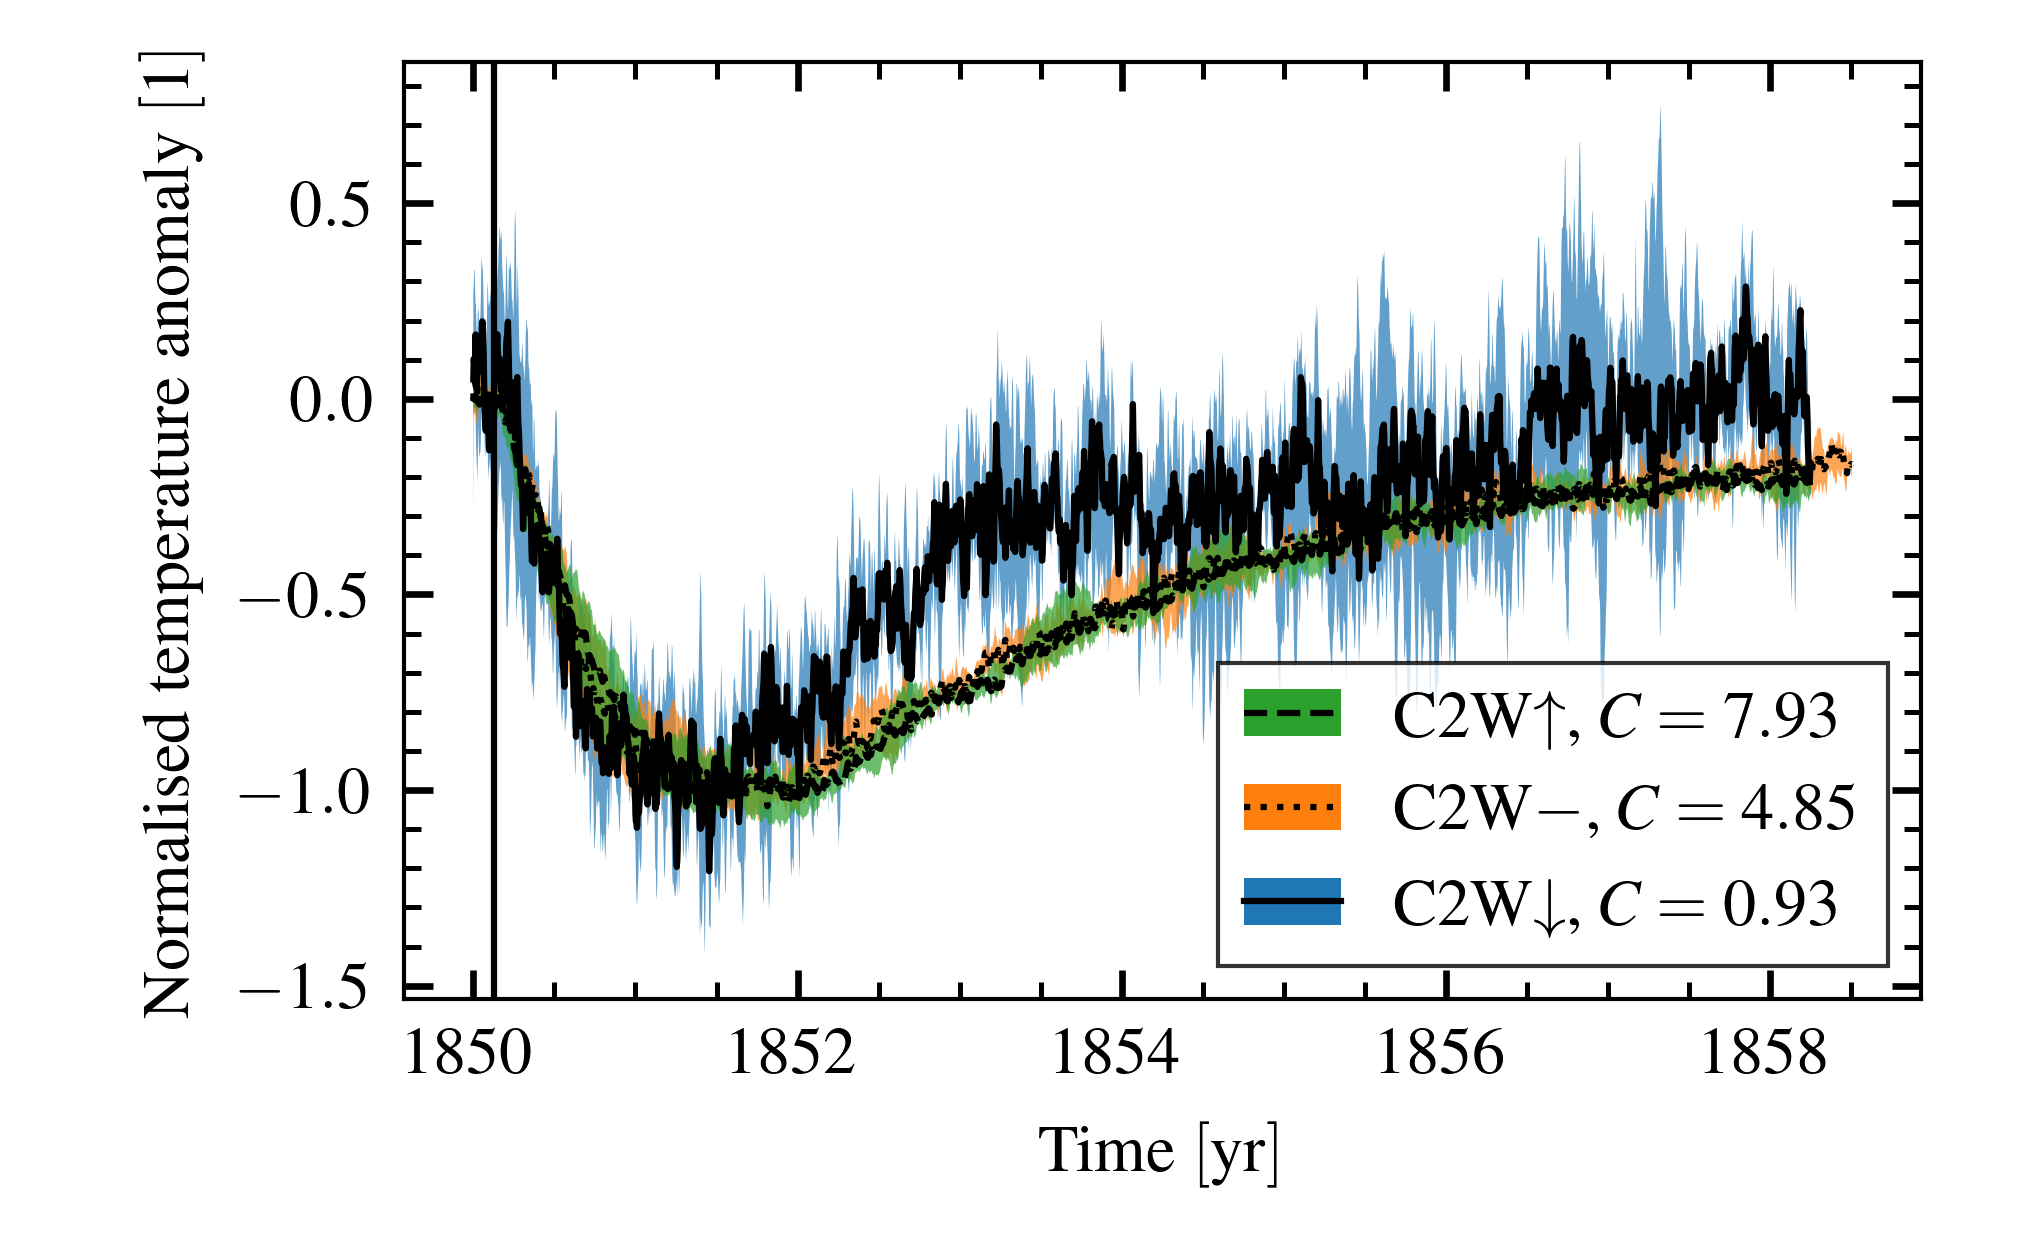
\includegraphics[width=0.95\linewidth]{figures/compare-waveform-max.png}
  \end{center}
  \caption{Normalized temperature response to three different-size volcanic eruptions,
    by setting a maximum peak value}%
  \label{fig:temp_norm_max}
\end{figure}

\begin{figure}[t]
  \begin{center}
    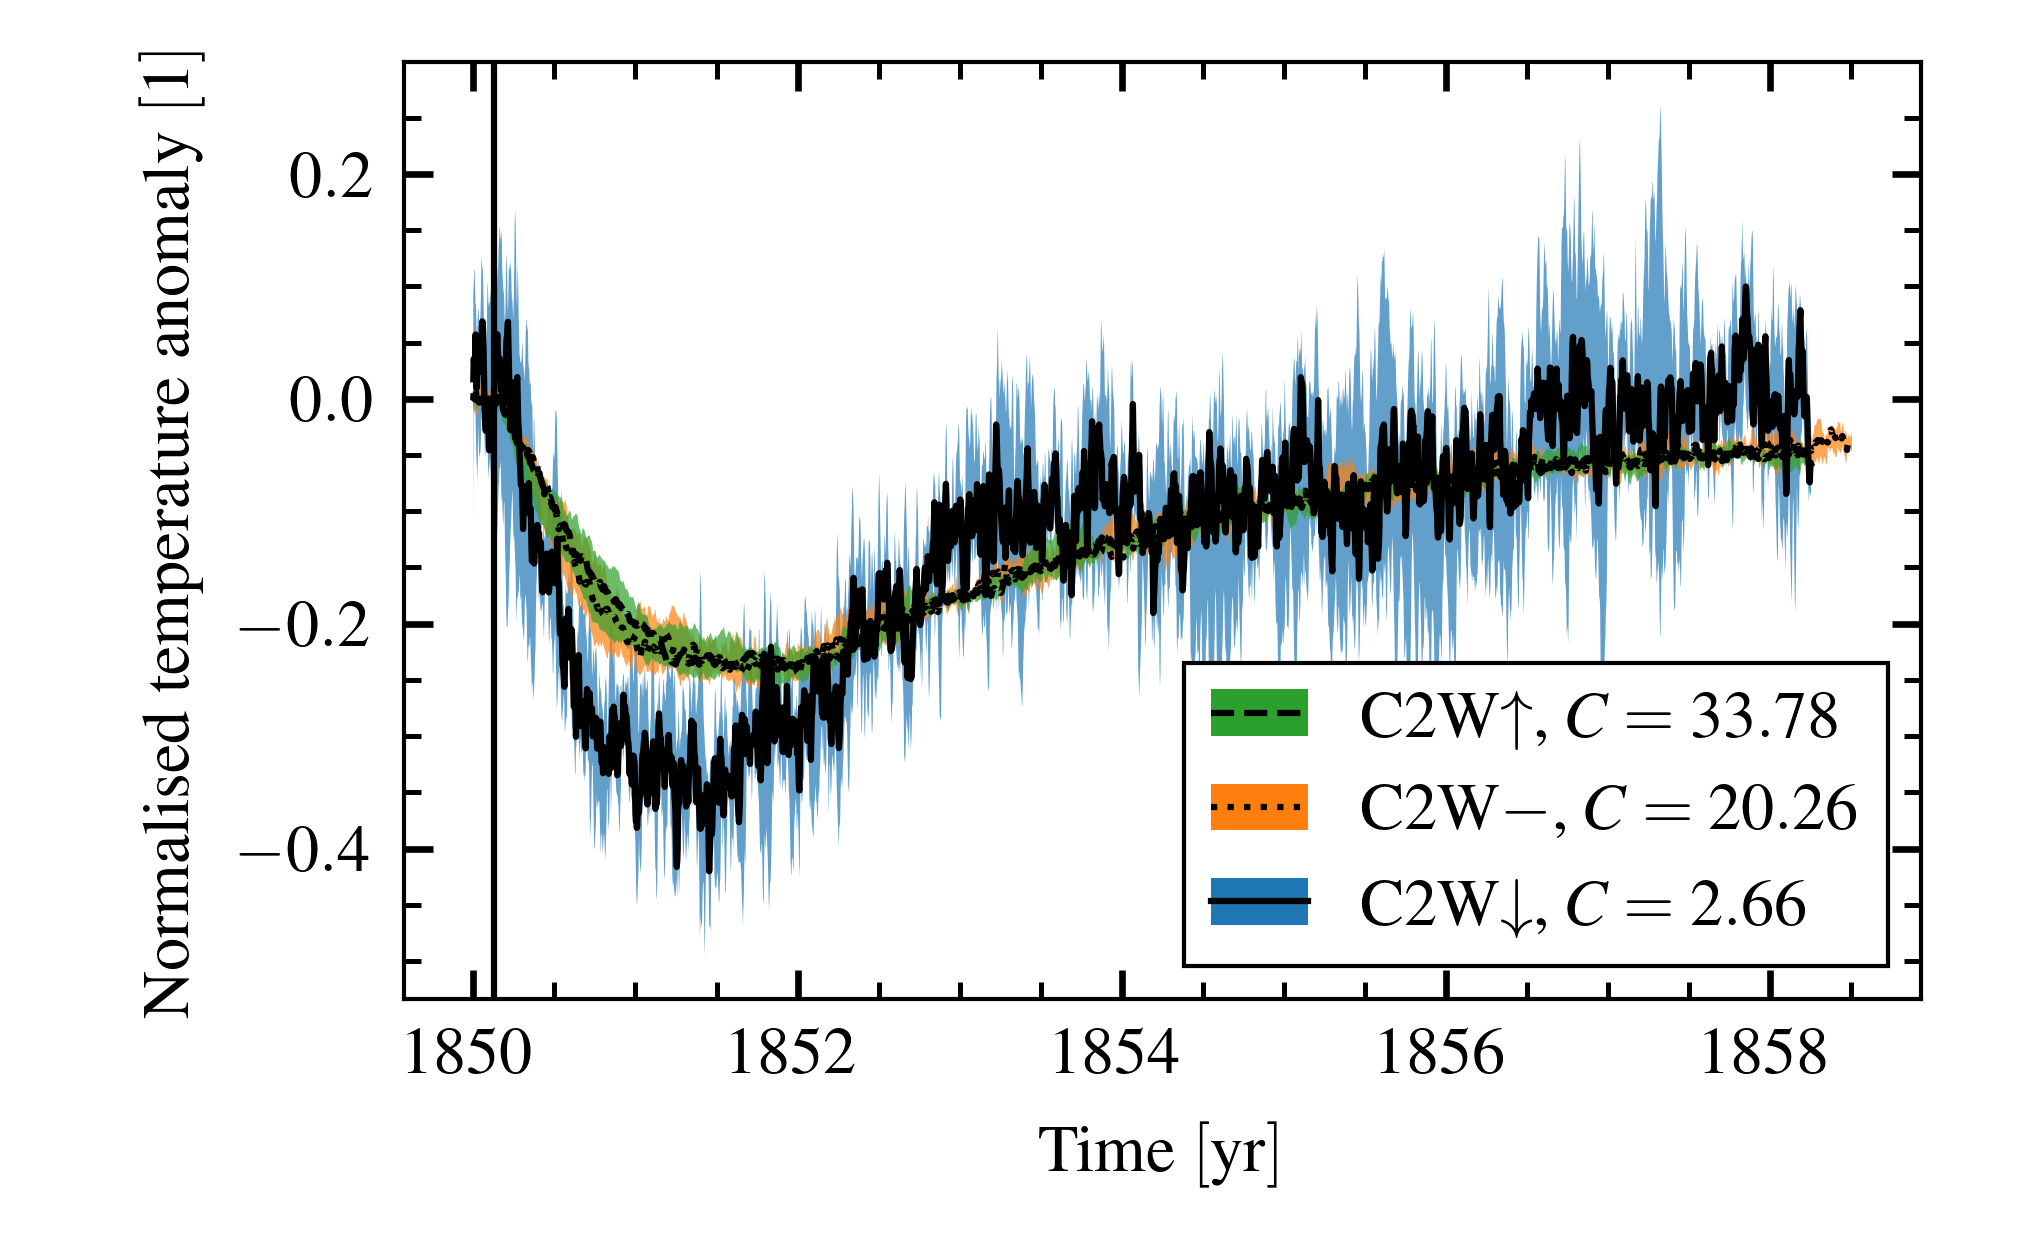
\includegraphics[width=0.95\linewidth]{figures/compare-waveform-integrate.png}
  \end{center}
  \caption{Normalized temperature response to three different-size volcanic eruptions,
    using integration, i.e., they all integrate to one}%
  \label{fig:temp_norm_int}
\end{figure}

\subsection{Parameter scan}

Whether the temperature time series have different shape depending on forcing strength
or not is a natural next step to take, and we here look more closely into the different
forcings. This comparison is also motivated by \citet{gregory2016}, specifically their
figure 4 which compare annual mean \acrfull{aod} with \acrfull{rf}.
\Cref{fig:aod_vs_toa_full} show annual mean values from the three simulation cases along
with the gradient obtained by \citet{gregory2016} of \(-19\). The annual mean data from
the smallest Pinatubo-like eruption (blue downward facing triangles,
\cref{fig:aod_vs_toa_inset}) has \acrshort{rf} values compared to \acrshort{aod} that
nicely follow the same constant gradient as the \citet{gregory2016} data used in their
figure 4.

However, we do find that the stronger eruptions lead to very different responses in
\acrshort{aod} and \acrshort{rf}, where the slope of the intermediate seem to follow
close to a \( -10 \) gradient and the strong is closer to a \( -4 \) gradient. The peak
values (red circles) suggest a logarithmic looking functional shape dependence, while
within each eruption strength the annual mean values fall relatively close to on a
straight line, but does tend to draw an elongated loop. This is the case also for the
small eruption strength shown in \cref{fig:aod_vs_toa_inset}.

Focusing on the peaks as shown by the red circles, previous papers simulating similar
effects have found the same trend. \citet{niemeier2015} did simulations of continually
emitting injections of sulphur, up to \( \SI{100}{\tera\gram
  \mathrm{(S)}\mathrm{yr}^{-1}} \), and found that the impact of increasing the injection
rate lead to a radiative forcing as a function of injection rate that had an exponential
decay and that converged to \( \SI{-65}{\watt\meter^{-2}} \)
\begin{equation}
  \Delta
  R_{\mathrm{TOA}} =
  -\SI{65}{\watt\metre^{-2}}
  \mathrm{e}^{-\left(\frac{\SI{2246}{\tera\gram(S)yr^{-1}}}{x}\right)^{0.23}}.
  \label{eq:niemeier_exponential}
\end{equation}
This upper limit is close to what one might suspect the \acrshort{cesm2} peaks and the
\acrfull{p100} simulation peak to approach (pink square in \cref{fig:aod_vs_toa_full}),
however, the functional shape is very different; the exponential found by
\citet{niemeier2015} have a much slower decay than what the \acrshort{cesm2} and
\acrshort{p100} data might follow. Given the very different scenarios; a constant level
of \iso{} in contrast to a specified injected mass simulating a volcanic eruption, it
should not be too surprising that the responses are different.

\begin{figure}[t]
  \begin{center}
    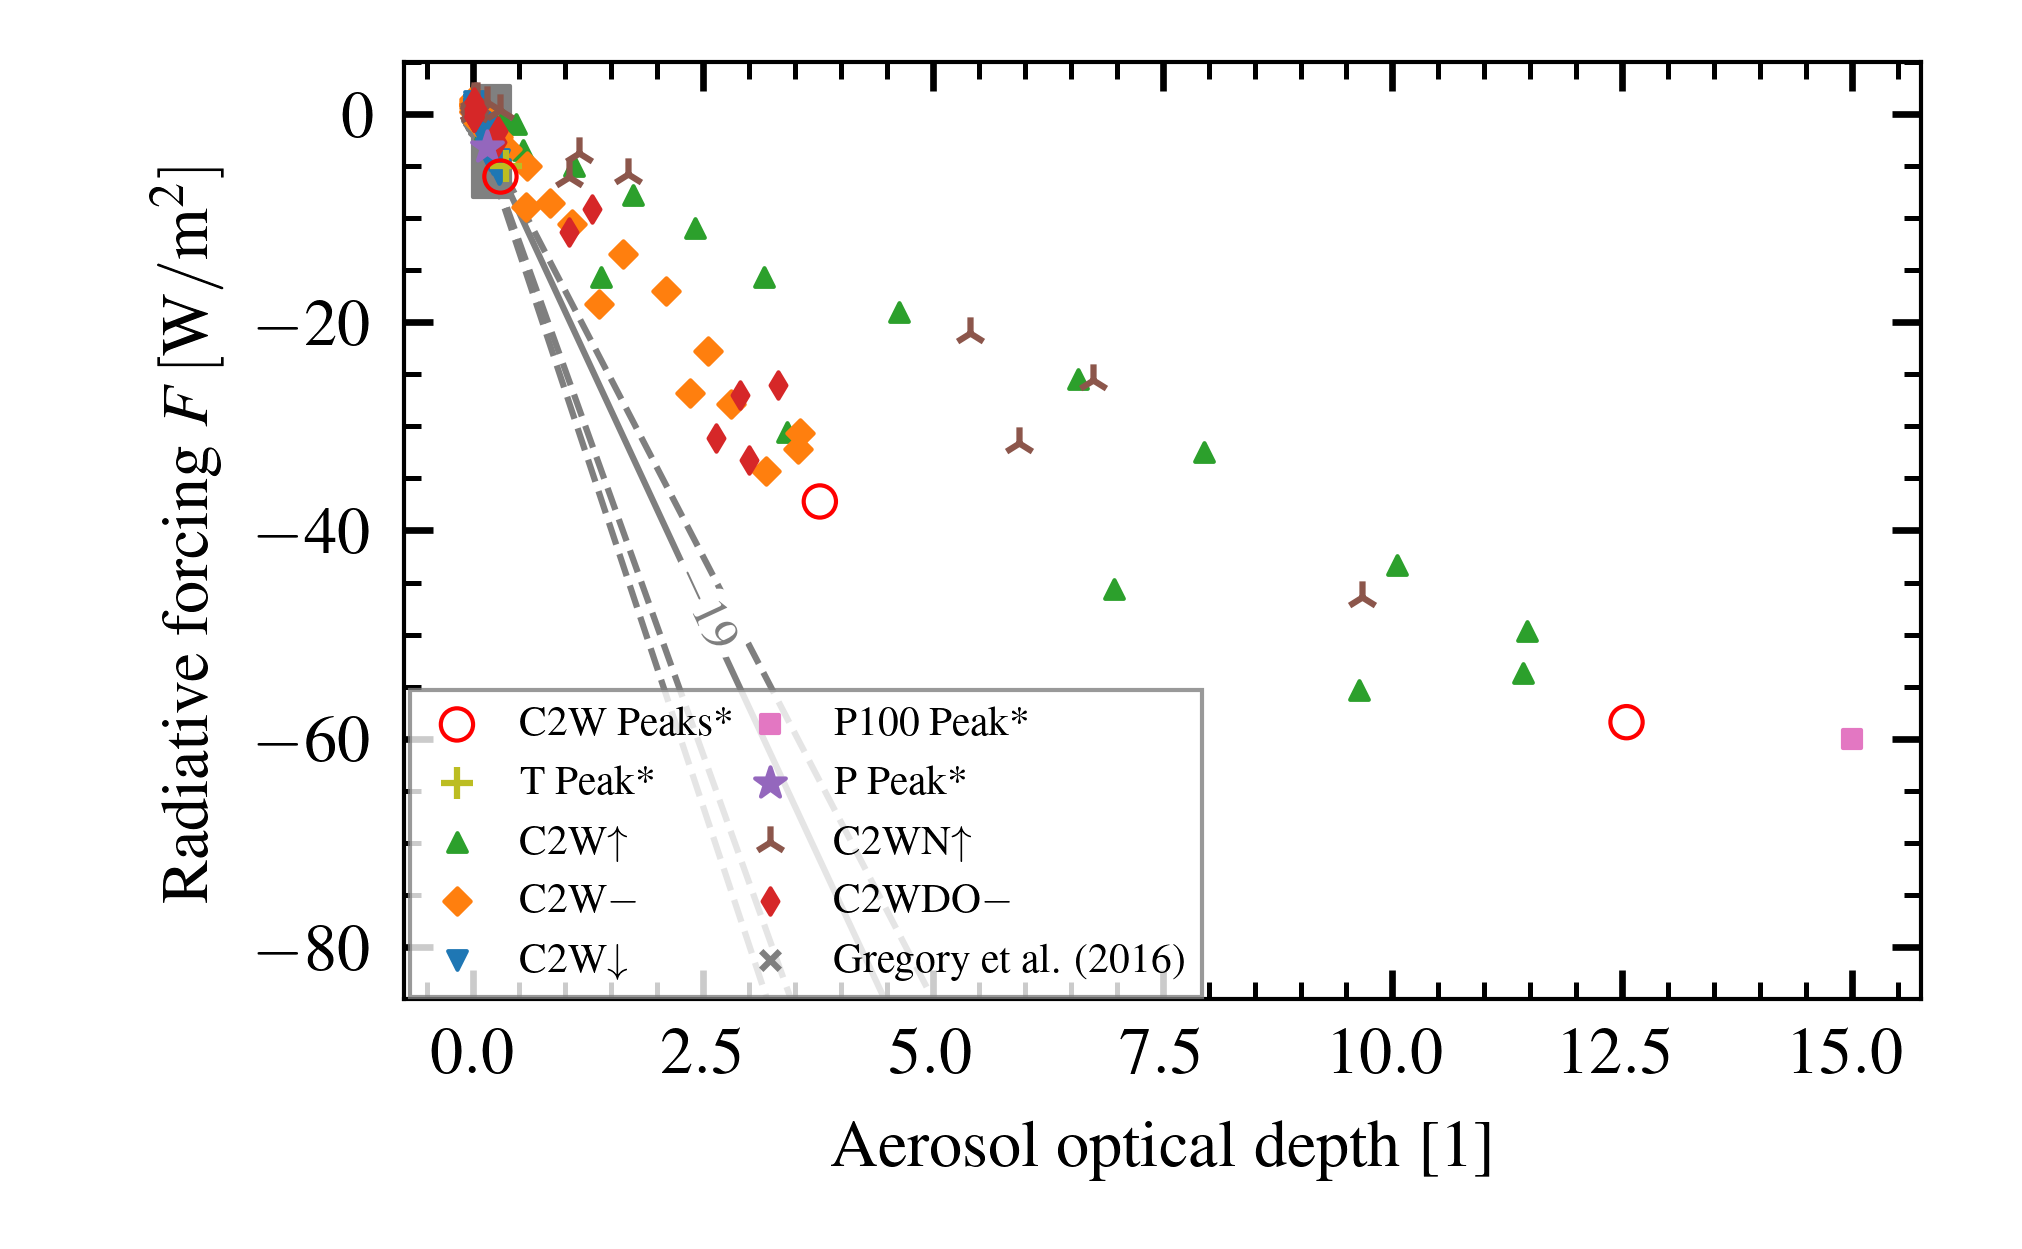
\includegraphics[width=0.95\linewidth]{figures/aod_vs_toa_avg_full.png}
  \end{center}
  \caption{\acrshort{aod} versus \acrshort{rf}, full size. Same type as
    \citet{gregory2016}}%
  \label{fig:aod_vs_toa_full}
\end{figure}

\begin{figure}[t]
  \begin{center}
    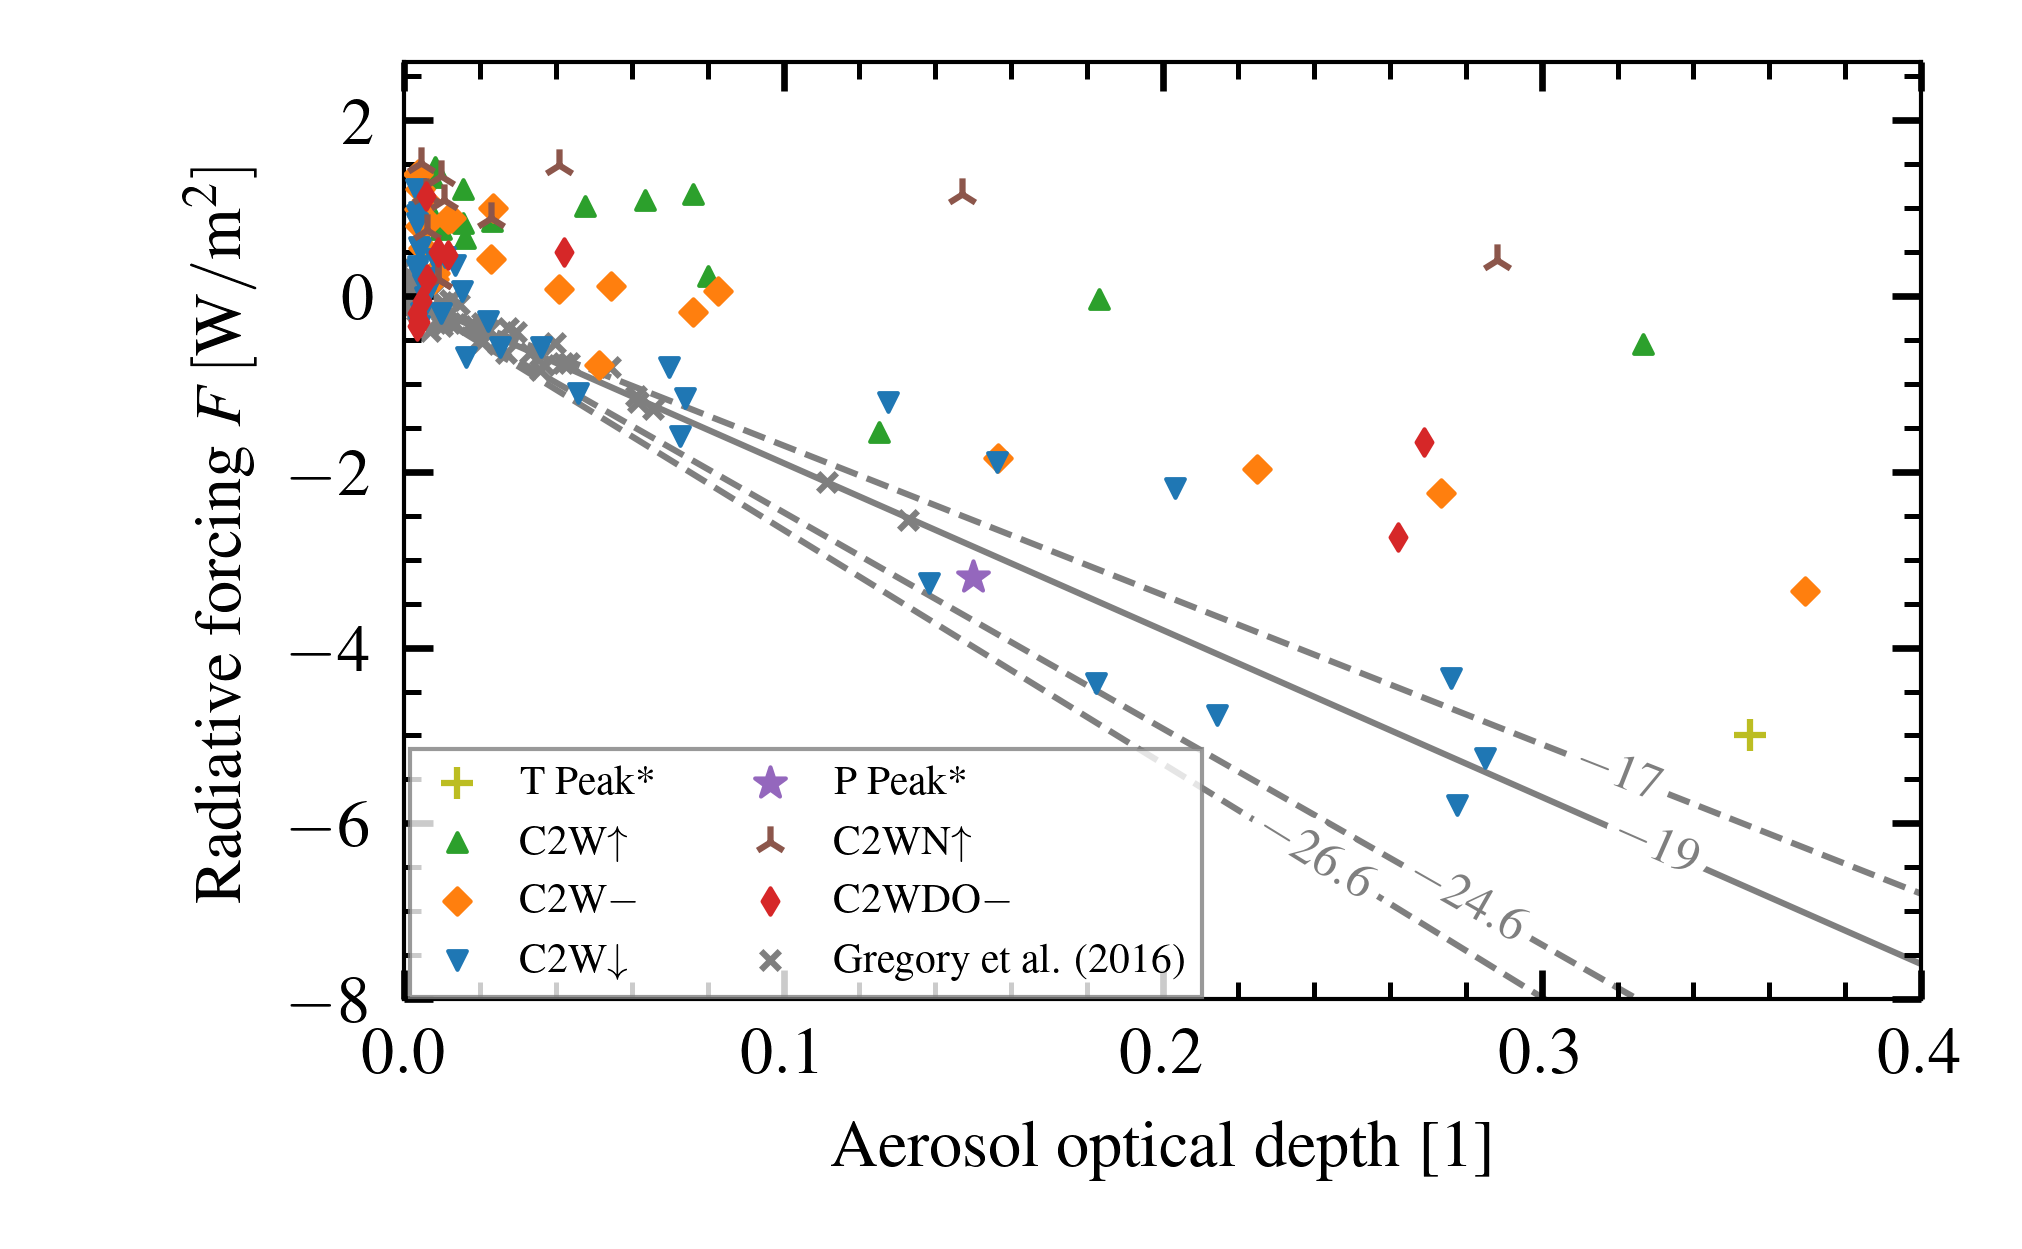
\includegraphics[width=0.95\linewidth]{figures/aod_vs_toa_avg_inset.png}
  \end{center}
  \caption{\acrshort{aod} versus \acrshort{rf}, inset. Same type as
    \citet{gregory2016}}%
  \label{fig:aod_vs_toa_inset}
\end{figure}

% \begin{figure}
%   \begin{center}
%     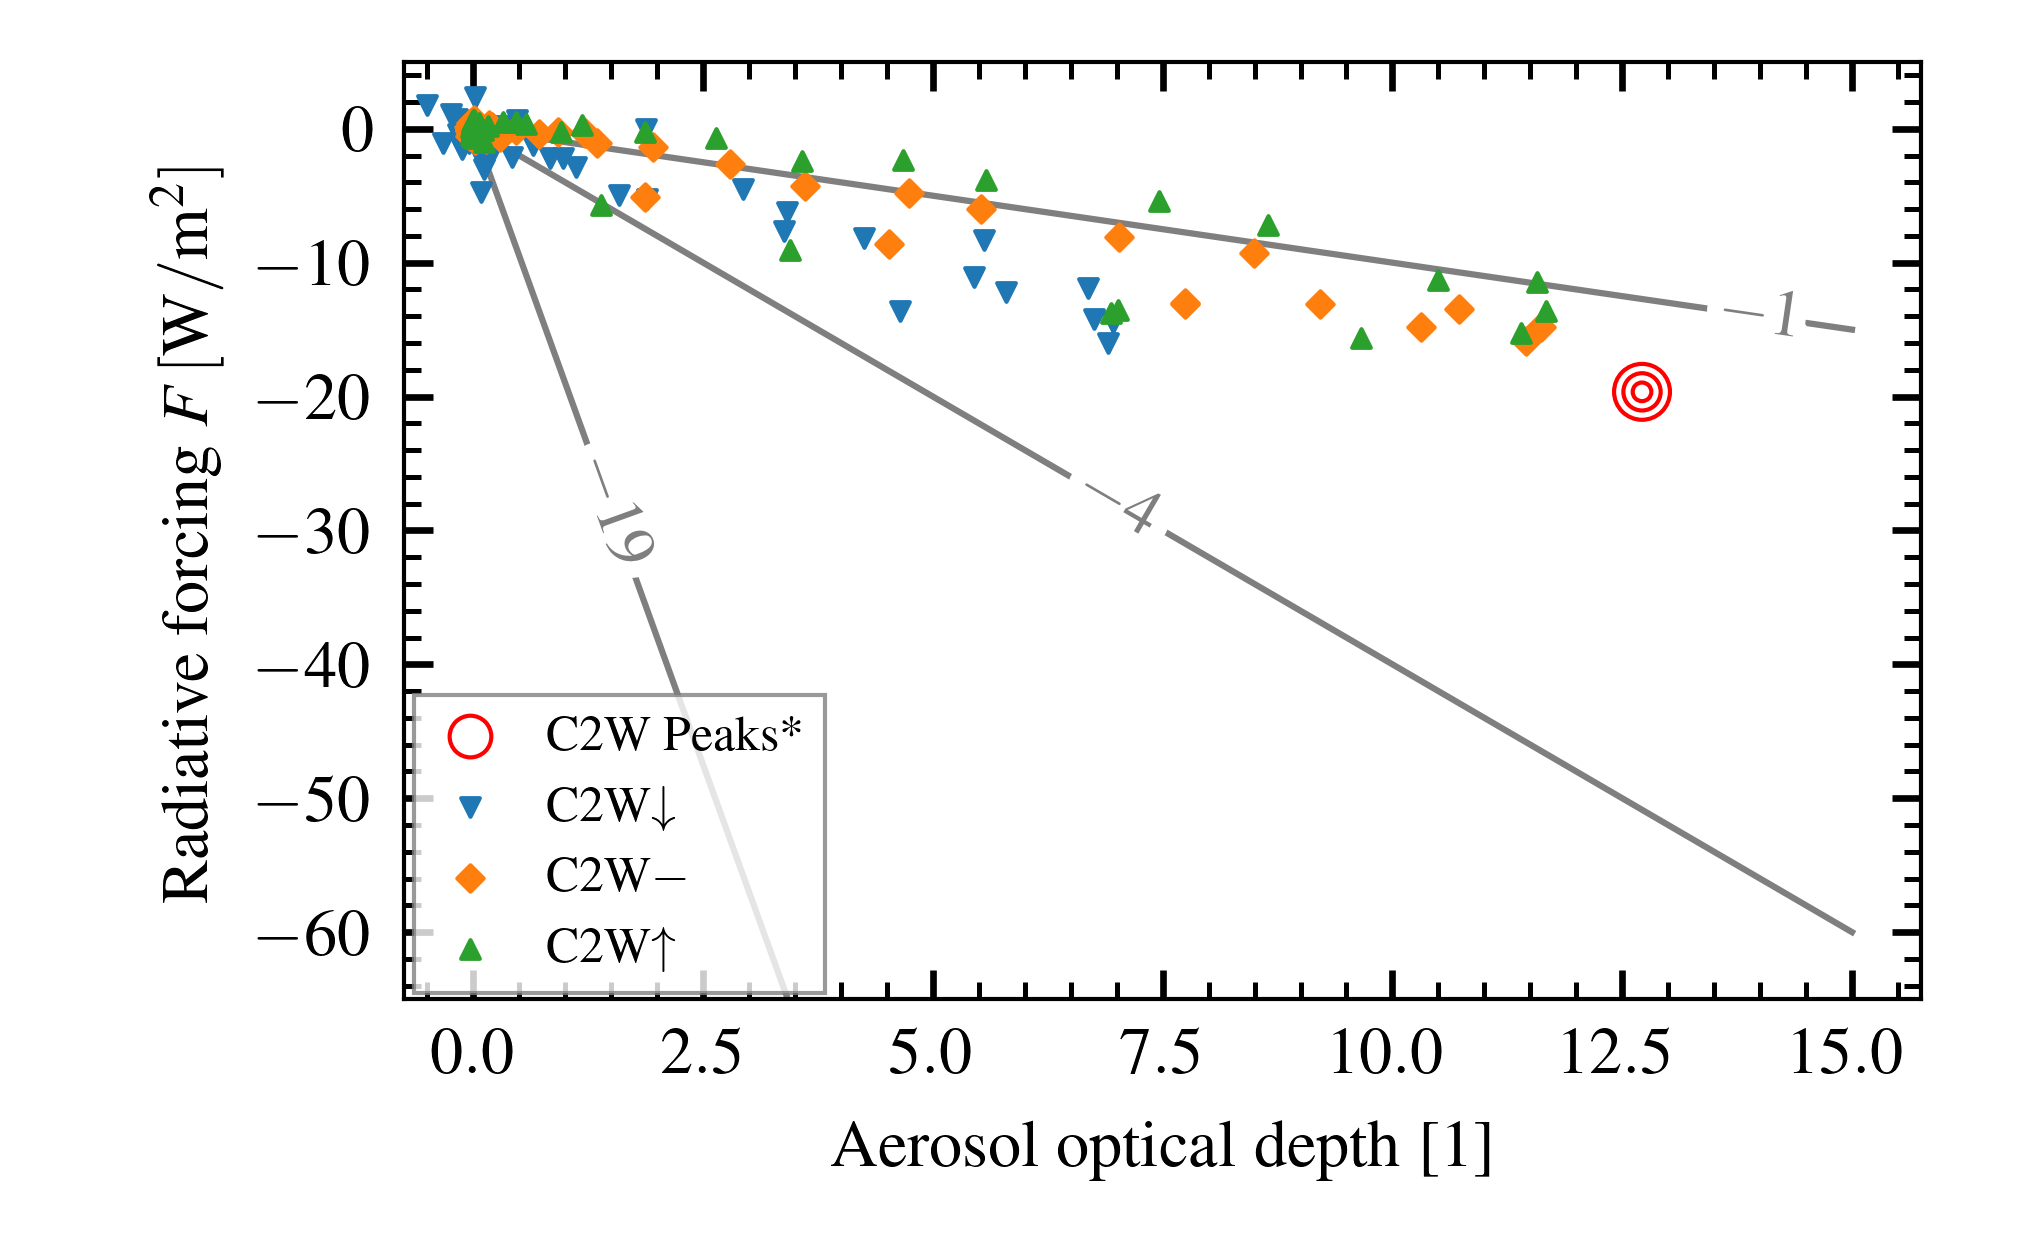
\includegraphics[width=0.95\linewidth]{figures/aod_vs_toa_avg_scaled.png}
%   \end{center}
%   \caption{
%     \acrshort{aod} versus \acrshort{rf}, scaled so the peak values of the different
%     volcano magnitudes are aligned. Same type as \citet{gregory2016}
%   }%
%   \label{fig:aod_vs_toa_scaled}
% \end{figure}

\subsection{Forcing efficiency}

To further look into the responses in \acrshort{aod} and \acrshort{rf} due to the
differently sized volcanic eruptions, we plot in
\cref{fig:aod_vs_toa_avg_loop,fig:aod_vs_toa_avg_loop_scaled,fig:aod_vs_toa_avg_loop_ratio,fig:aod_vs_toa_avg_loop_ratio_scaled}
seasonal means where the start of the time series are shifted so that the eruption day
is at time zero, and all time series are exactly four years long.

% TODO: get out the three aerosol components to check growth and sedimentation

The ratio between \acrshort{aod} and \acrshort{rf} is not constant, but what is more is
that their ratio seem to draw a loop. Especially when the eruptions are very large,
\citet[][see their sections 3.1.2, 3.2.2]{marshall2019} describe how the growth of
aerosol particles affect both parameters. They introduce a suggested two phases of the
aerosol evolution, a ``growth'' phase and a ``sedimentation'' phase. In general there
are larger aerosols for larger eruptions (more time to grow), such that both
\acrshort{aod} and \acrshort{rf} will be weaker (they fall out due to gravity faster and
are less efficient at scattering radiation). In the later phase (``sedimentation''
phase) \acrshort{rf} become more weak compared to \acrshort{aod} since, in addition to a
faster sedimentation rate, the \acrshort{rf} is further reduced due to the larger
aerosols being less effective at scattering \acrshort{sw} radiation. This is largely in
line with the results in
\cref{fig:aod_vs_toa_avg_loop,fig:aod_vs_toa_avg_loop_scaled,fig:aod_vs_toa_avg_loop_ratio,fig:aod_vs_toa_avg_loop_ratio_scaled},
where (1) the larger eruptions have a smaller ratio (larger aerosols scatter
\acrshort{sw} radiation more poorly) and (2) the ratio is decreasing in magnitude as the
eruption evolve (in the early phase only, the later phase give a roughly constant ratio,
see \cref{fig:aod_vs_toa_avg_loop_ratio}). Based on the simple two phases of the aerosol
evolution \citep{marshall2019}, an increasing \acrshort{rf} to \acrshort{aod} ratio
(decreasing when considering absolute values) seems reasonable.

\citet[][their figure 1c,d]{marshall2020} present results showing a time dependence
in the conversion between \acrshort{saod} and \acrshort{rf}, but where
\acrshort{rf} should be larger later in the eruption evolution when compared to
\acrshort{aod}, not weaker. This happen since the aerosols are initially spatially
confined to the hemisphere where the eruption was at before it spread, leading to a
larger global mean albedo per \acrshort{saod} and in turn large \acrshort{rf} per
\acrshort{saod} \citep{marshall2020}. From their results and the results shown here in
\cref{fig:aod_vs_toa_avg_loop,fig:aod_vs_toa_avg_loop_scaled,fig:aod_vs_toa_avg_loop_ratio,fig:aod_vs_toa_avg_loop_ratio_scaled},
there seems to be several and competing effects that decide on the values of
\acrshort{saod} and \acrshort{rf}.

% FIX: Marshall et al. 2020 used 1-e^{-SAOD}, so check this out as well.

\begin{figure}[t]
  \begin{center}
    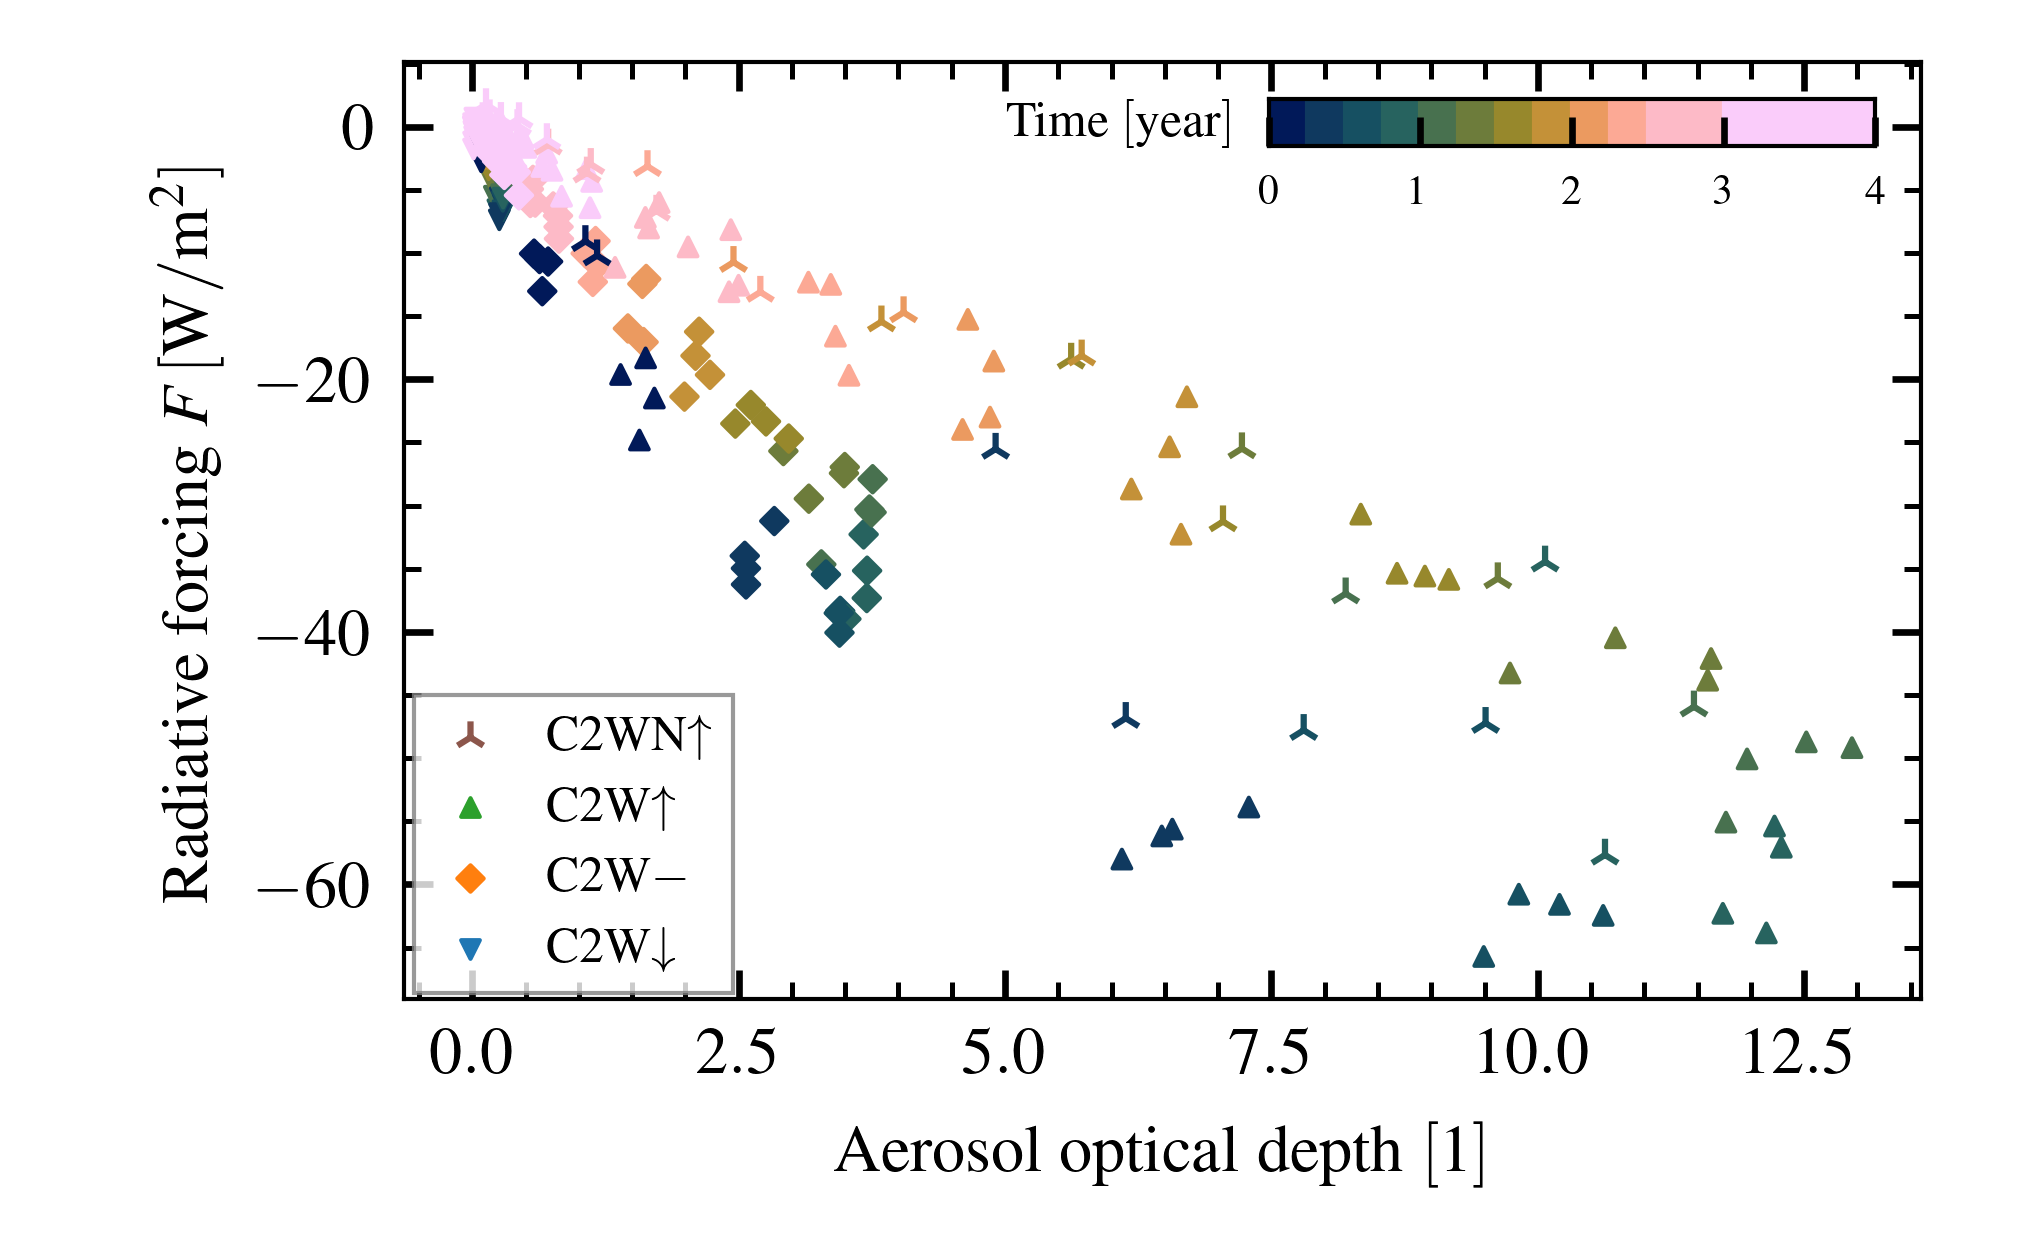
\includegraphics[width=0.95\linewidth]{figures/aod_vs_toa_avg_loop.png}
  \end{center}
  \caption{
    \acrshort{aod} versus \acrshort{rf}, with points coloured according to the year and
    season it was averaged from. (Same type of plot as \citet{gregory2016})
  }%
  \label{fig:aod_vs_toa_avg_loop}
\end{figure}

\begin{figure}[t]
  \begin{center}
    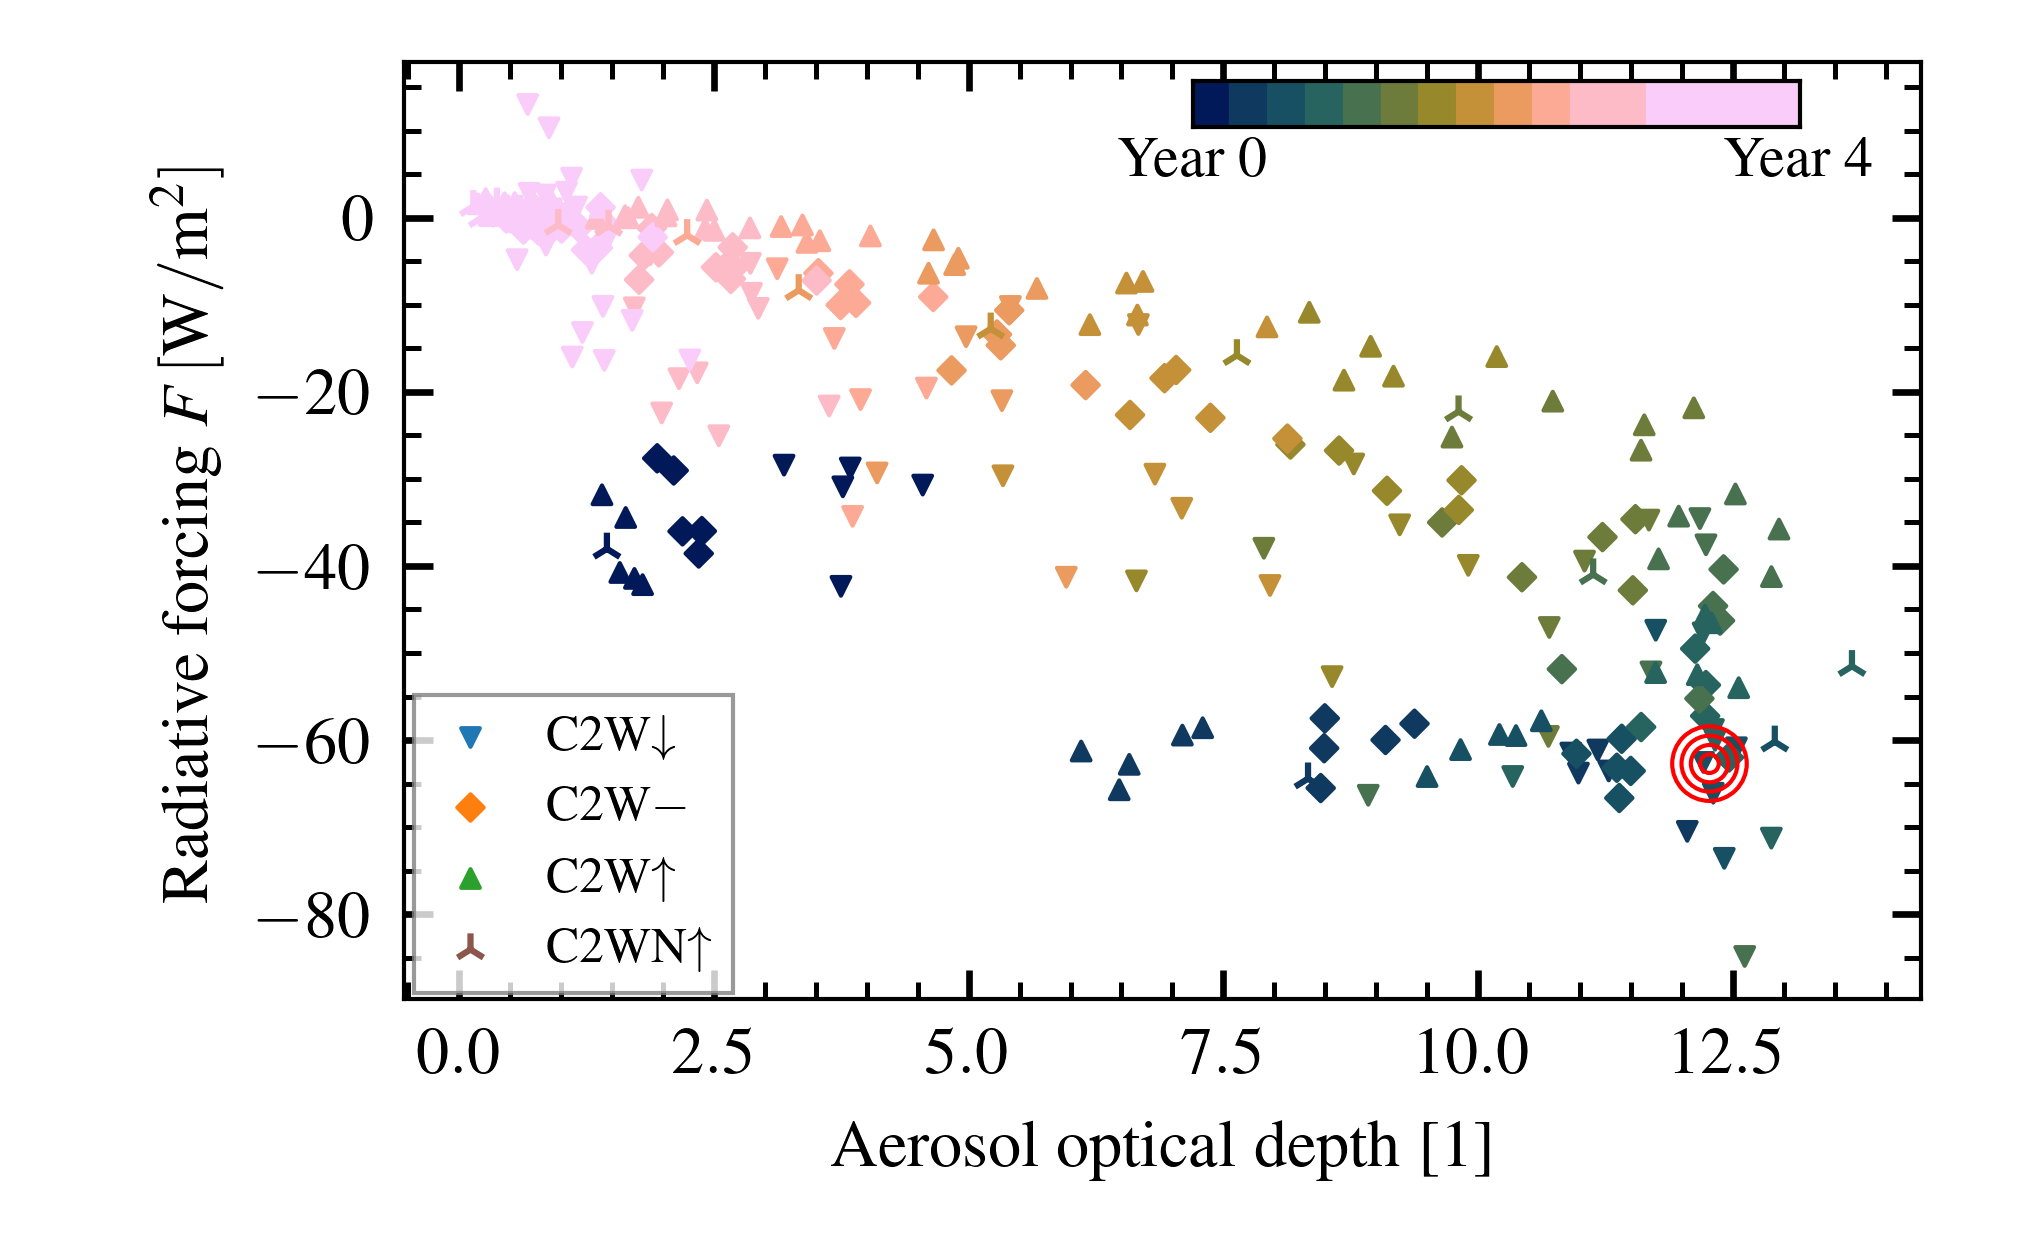
\includegraphics[width=0.95\linewidth]{figures/aod_vs_toa_avg_loop_scaled.png}
  \end{center}
  \caption{
    \acrshort{aod} versus \acrshort{rf}, with points coloured according to the year and
    season it was averaged from, and scaled so the peak values are aligned. (Same type
    of plot as \citet{gregory2016})
  }%
  \label{fig:aod_vs_toa_avg_loop_scaled}
\end{figure}

In \cref{fig:aod_vs_toa_avg_loop_ratio} we plot the ratio of the annual means of
\acrshort{rf} and \acrshort{aod}. The years where the signal-to-noise ratio is best is
in years 1 and 2, as well as year 0 (the noise is mostly due to the \acrshort{rf} time
series, shown in \cref{fig:toa_arrays_normalized}). For this reason, the ratio of
\acrshort{rf} to \acrshort{aod} is calculated for the second season of the first year
until the end of the third year. From this we find that even though the ratio changes
between the eruption magnitudes, we do find that the gradient at which the ratio is
changing is similar across large eruption magnitudes. A slope of approximately \( 5.8 \)
is a good fit for both the intermediate (orange thick diamonds) and the strong eruption
(green upward triangles), and even though the spread in the small eruption (blue
downward triangles) is large in the \( y \)-direction, they tend to follow a similarly
inclined, albeit steeper, slope. In the later phase, from the second season of the
second year, the ratios stay close to constant for the reminder of the decaying phase.

The change in ratio, where the smallest is found in the strong eruption and the largest
ratio is from the small eruption, is consistent with the change in peak values seen in
\cref{fig:aod_vs_toa_full}, where the red circles show the peak values are bending off
to the right. The \acrshort{rf} increase in magnitude slows down while \acrshort{aod}
increases close to linearly with injected \ce{SO2} (see also \cref{fig:so2_vs_aod}).
This could be the result of larger aerosols having time to develop as the amount of
injected \ce{SO2} increase \citep{niemeier2015,marshall2019}. This in turn make the
forcing from smaller eruptions relatively more efficient than from large eruptions since
larger aerosols scatter radiation less efficiently, causing a larger ratio between
\acrshort{rf} and \acrshort{aod}.

\begin{figure}[t]
  \begin{center}
    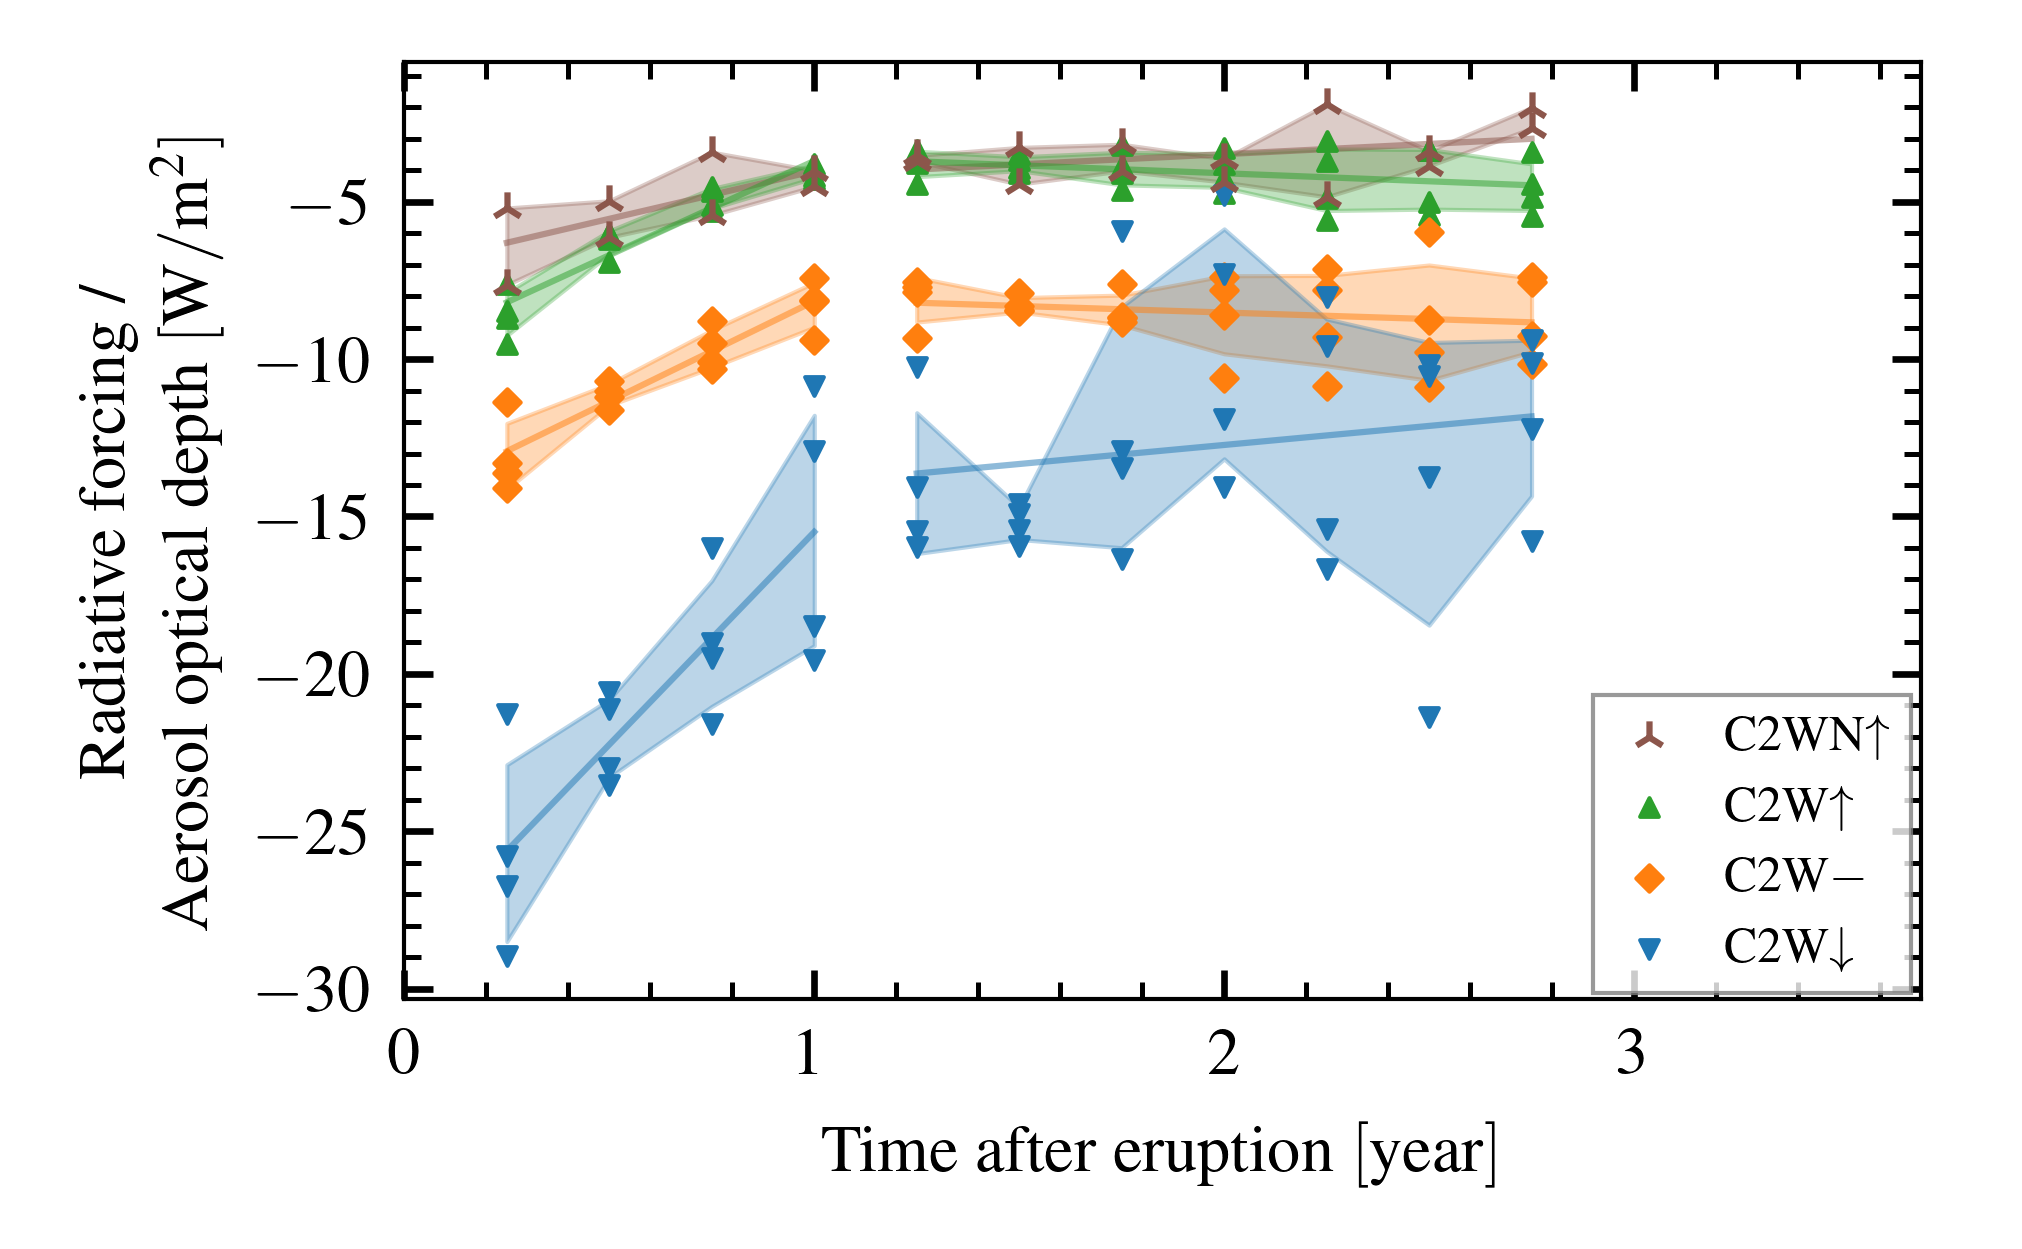
\includegraphics[width=0.95\linewidth]{figures/aod_vs_toa_avg_loop_ratio.png}
  \end{center}
  \caption{
    Ratio of \acrshort{rf} to \acrshort{aod} as shown in
    \cref{fig:aod_vs_toa_avg_loop}, with the time-after-eruption on the horizontal axis.
    Slopes are linear regression fits using \textbf{scipy}
  }%
  \label{fig:aod_vs_toa_avg_loop_ratio}
\end{figure}

\begin{figure}[t]
  \begin{center}
    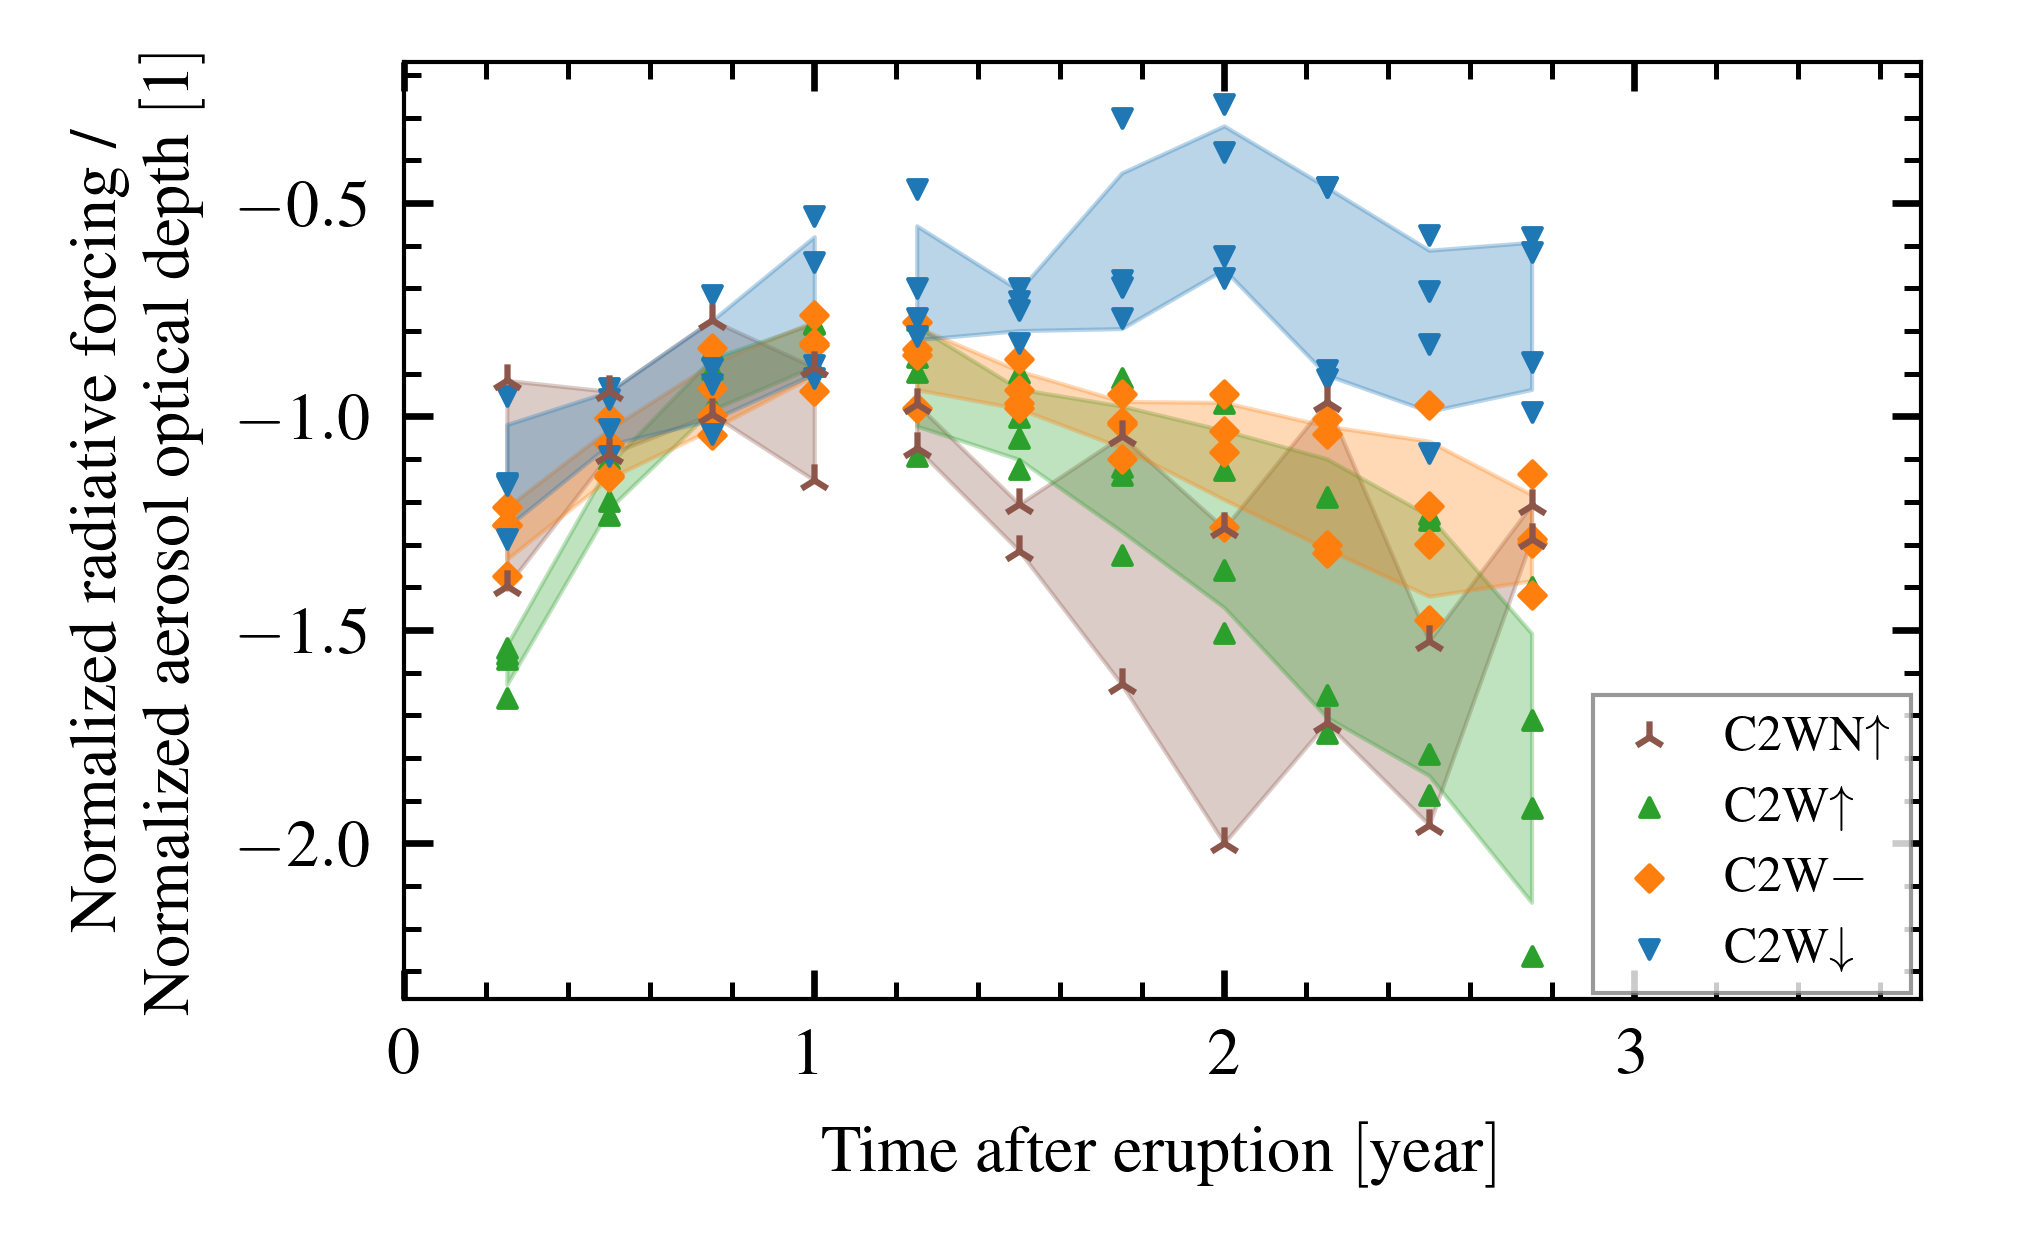
\includegraphics[width=0.95\linewidth]{figures/aod_vs_toa_avg_loop_ratio_scaled.png}
  \end{center}
  \caption{
    A scaled version of \cref{fig:aod_vs_toa_avg_loop_ratio}, where the scaling is the
    exact same as in \cref{fig:aod_vs_toa_avg_loop_scaled} compared to
    \cref{fig:aod_vs_toa_avg_loop}
  }%
  \label{fig:aod_vs_toa_avg_loop_ratio_scaled}
\end{figure}

One feature seen in \cref{fig:aod_vs_toa_avg_loop,fig:aod_vs_toa_avg_loop_ratio} is that
the early phase seem to have a \acrshort{rf} to \acrshort{aod} ratio that is changing
(from about \( 0 \) to \( 1.2 \) years after the eruption), while the later phase has an
almost constant ratio (from \( 1.2 \) to \( 3 \)--\( 4 \) years after the eruption).
When plotting the \acrshort{rf} time series we find that their shape is very consistent
over different eruption strengths (\cref{fig:toa_arrays_normalized}), but the
\acrshort{aod} time series show a slight change in shape from smaller to larger
eruptions (\cref{fig:aod_arrays_normalized}). Specifically, the \acrshort{aod} time
series from the smallest eruptions have a fast rise and a flat peak before it decays
back to its equilibrium state, while from the two larger eruptions we find a slower rise
time, but a sharper peak, making the decay to equilibrium happen at a similar time after
the eruption and at a similar rate.
% TODO: Why? Marshall et al. (2019) and references therein may be the best source for a
% suggested explanation.

An interesting aspect with the similar decaying phase seen in both the \acrshort{aod}
time series and the \acrshort{rf} time series is how this might influence the
temperature time series, and whether one would expect a similar trend in them. That is,
if one might expect the temperature time series to have different shape in the rising
phase, but similar shape in the decaying phase, as discussed in relation to
\cref{fig:temp_norm_max,fig:temp_norm_int}. Allowing the simulations to run for at least
twenty years to allow the tail to be well resolved is therefore another avenue that
could be explored further.

\begin{figure}[t]
  \begin{center}
    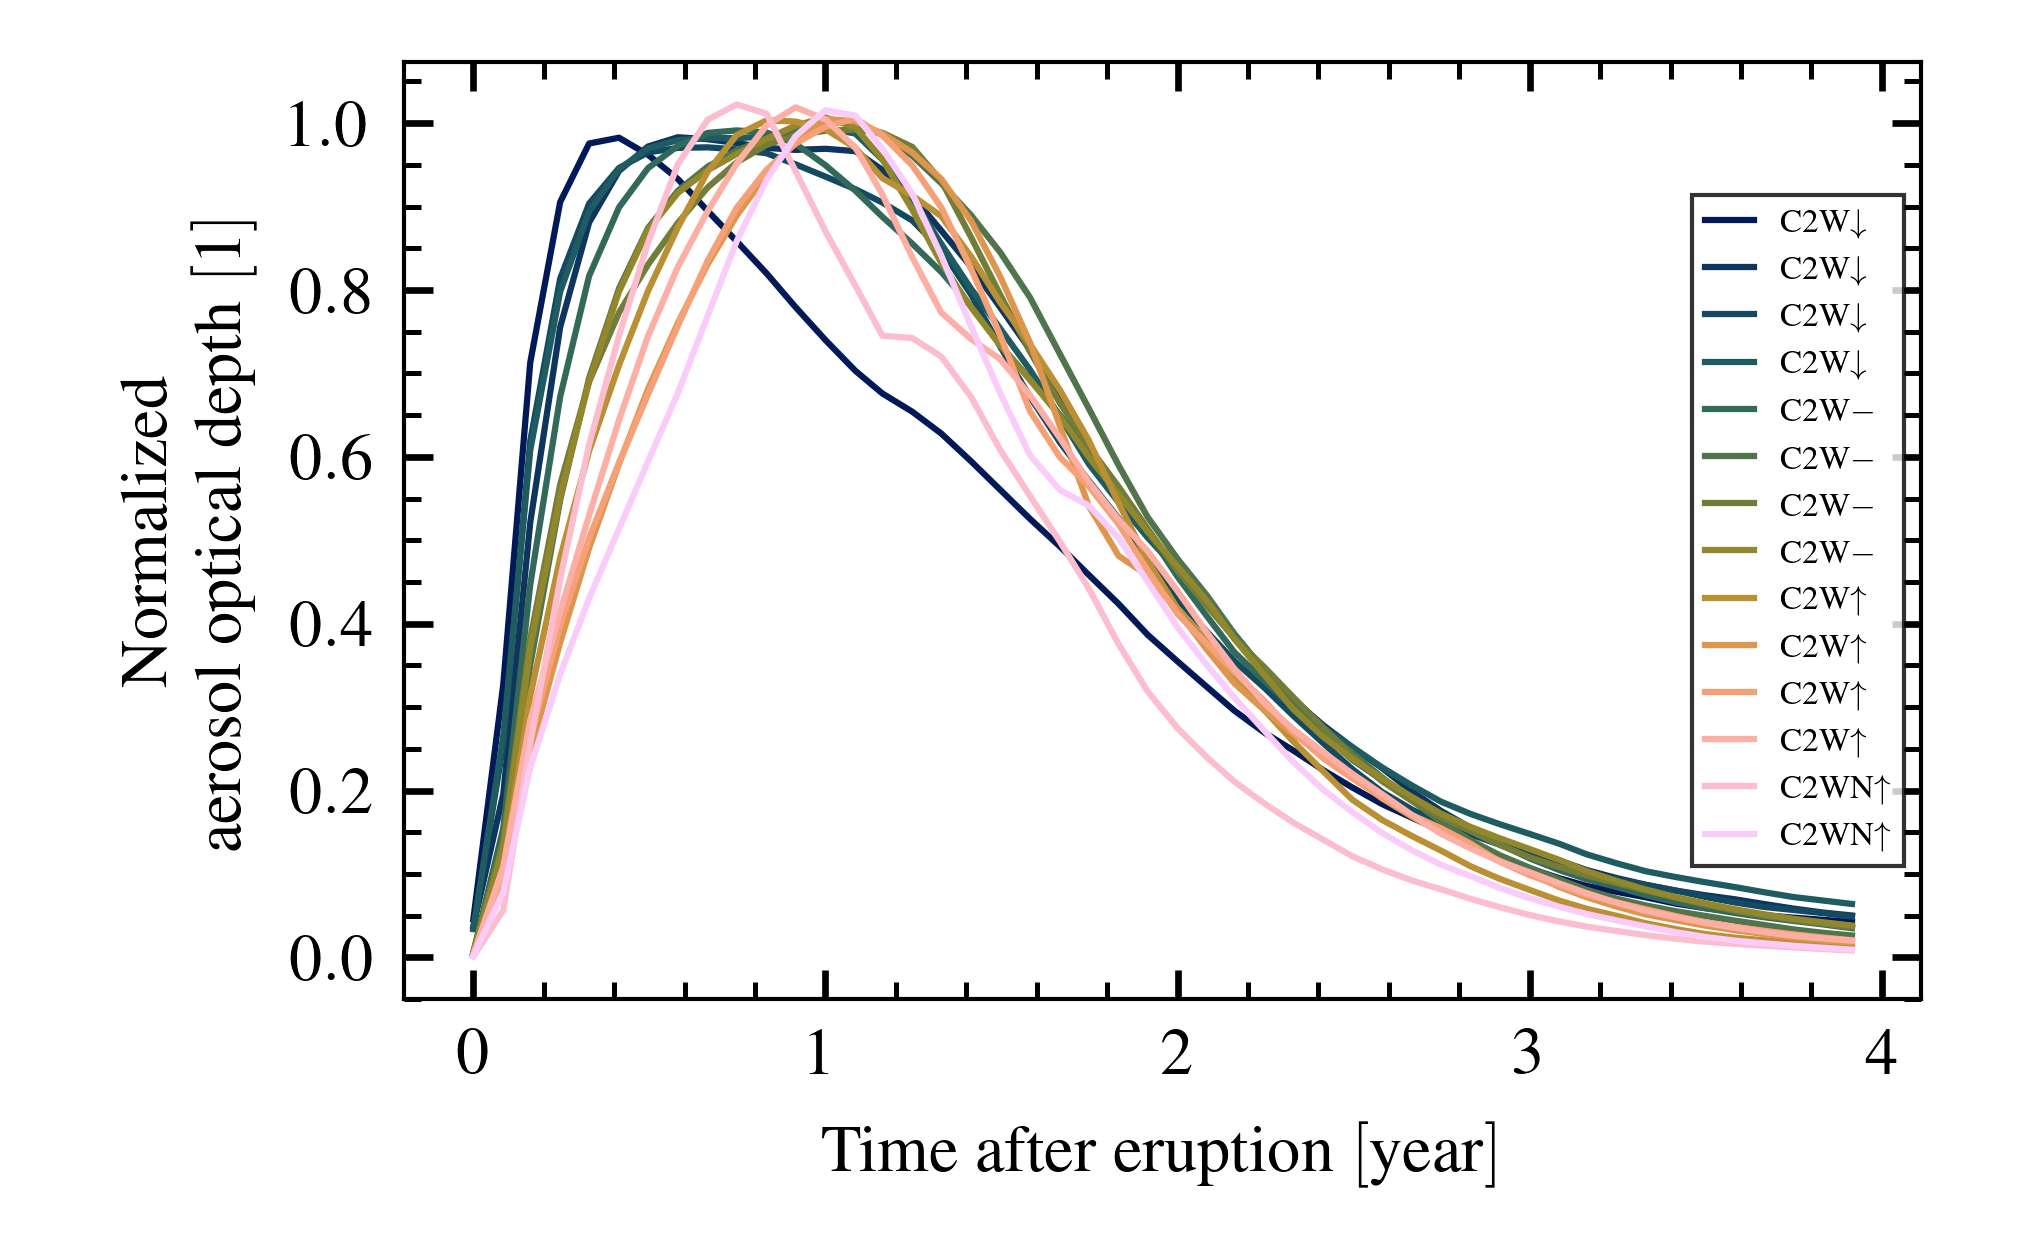
\includegraphics[width=0.95\linewidth]{figures/aod_arrays_normalized.png}
  \end{center}
  \caption{
    The (scaled versions of the) arrays used in
    \cref{fig:aod_vs_toa_avg_loop_scaled,fig:aod_vs_toa_avg_loop_ratio_scaled}
    (\cref{fig:aod_vs_toa_avg_loop,fig:aod_vs_toa_avg_loop_ratio})
  }%
  \label{fig:aod_arrays_normalized}
\end{figure}

\begin{figure}[t]
  \begin{center}
    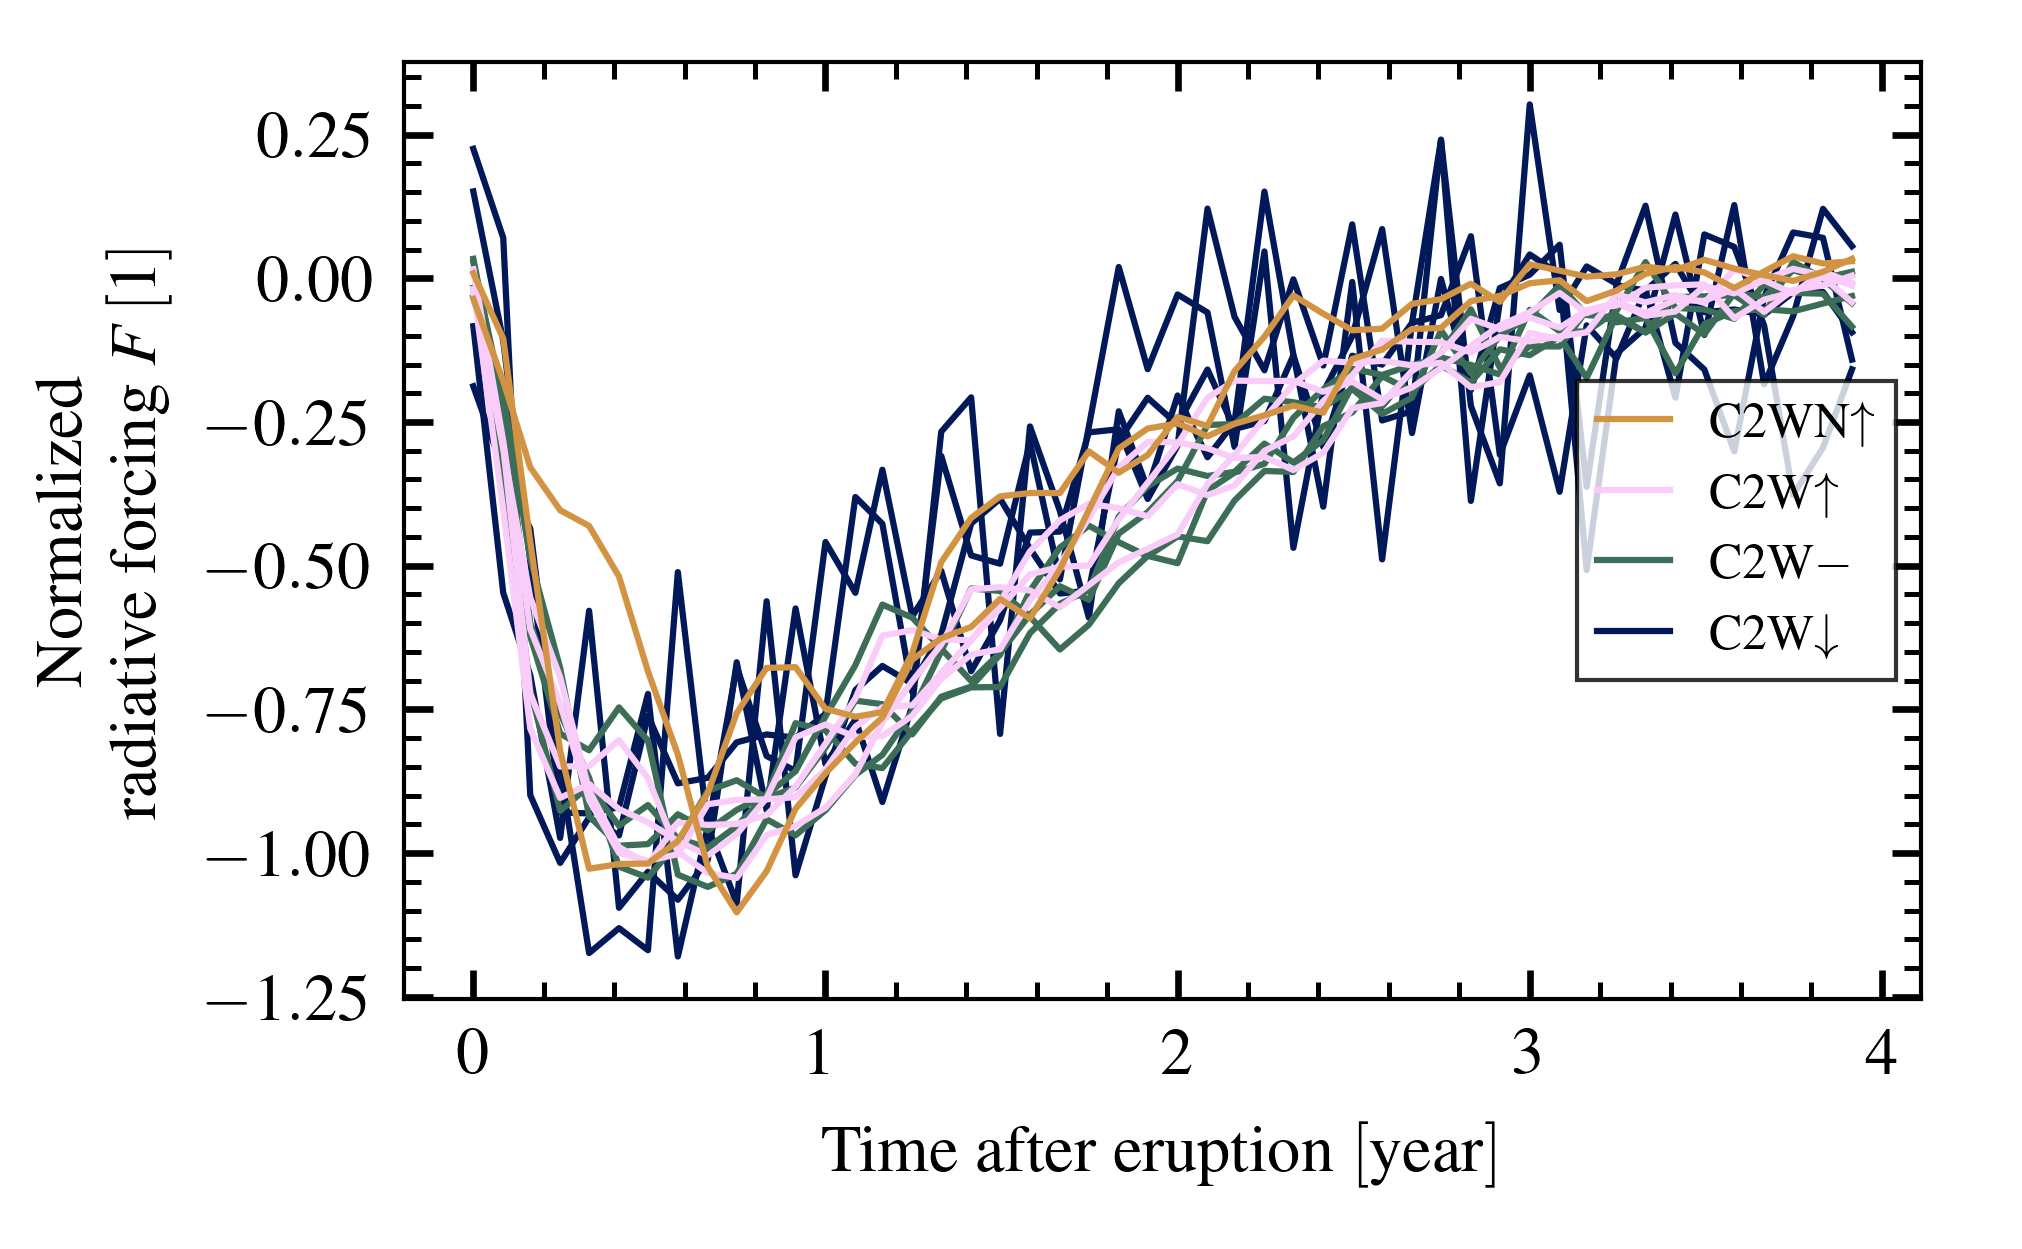
\includegraphics[width=0.95\linewidth]{figures/toa_arrays_normalized.png}
  \end{center}
  \caption{
    The (scaled versions of the) arrays used in
    \cref{fig:aod_vs_toa_avg_loop_scaled,fig:aod_vs_toa_avg_loop_ratio_scaled}
    (\cref{fig:aod_vs_toa_avg_loop,fig:aod_vs_toa_avg_loop_ratio})
  }%
  \label{fig:toa_arrays_normalized}
\end{figure}

\subsection{Comparing parameters}

Let us finally compare all relevant parameters to each other. The initial parameter that
is the input to the \acrshort{cesm2} is injected \ce{SO2}. Compared to \acrshort{aod} we
find that the \acrshort{cesm2} simulations result in an almost linear relationship
between them, shown in \cref{fig:so2_vs_aod}.\footnote{\emph{Since \iso{} is ``total
    amount of \iso{}'', maybe consider comparing to integrated values of \acrshort{aod},
    \acrshort{rf} and temperature as well, not just the peak values.}} The latitude also
play a role for how large the \acrshort{aod} perturbation become, as we can see from the
\textbf{C2WN\(\uparrow\)} data point, representing a strong eruption, but located at \(
\SI{56}{\degree N} \). The weak dependence on eruption latitude is also reported in
\citet{marshall2019}.

\begin{figure}[t]
  \begin{center}
    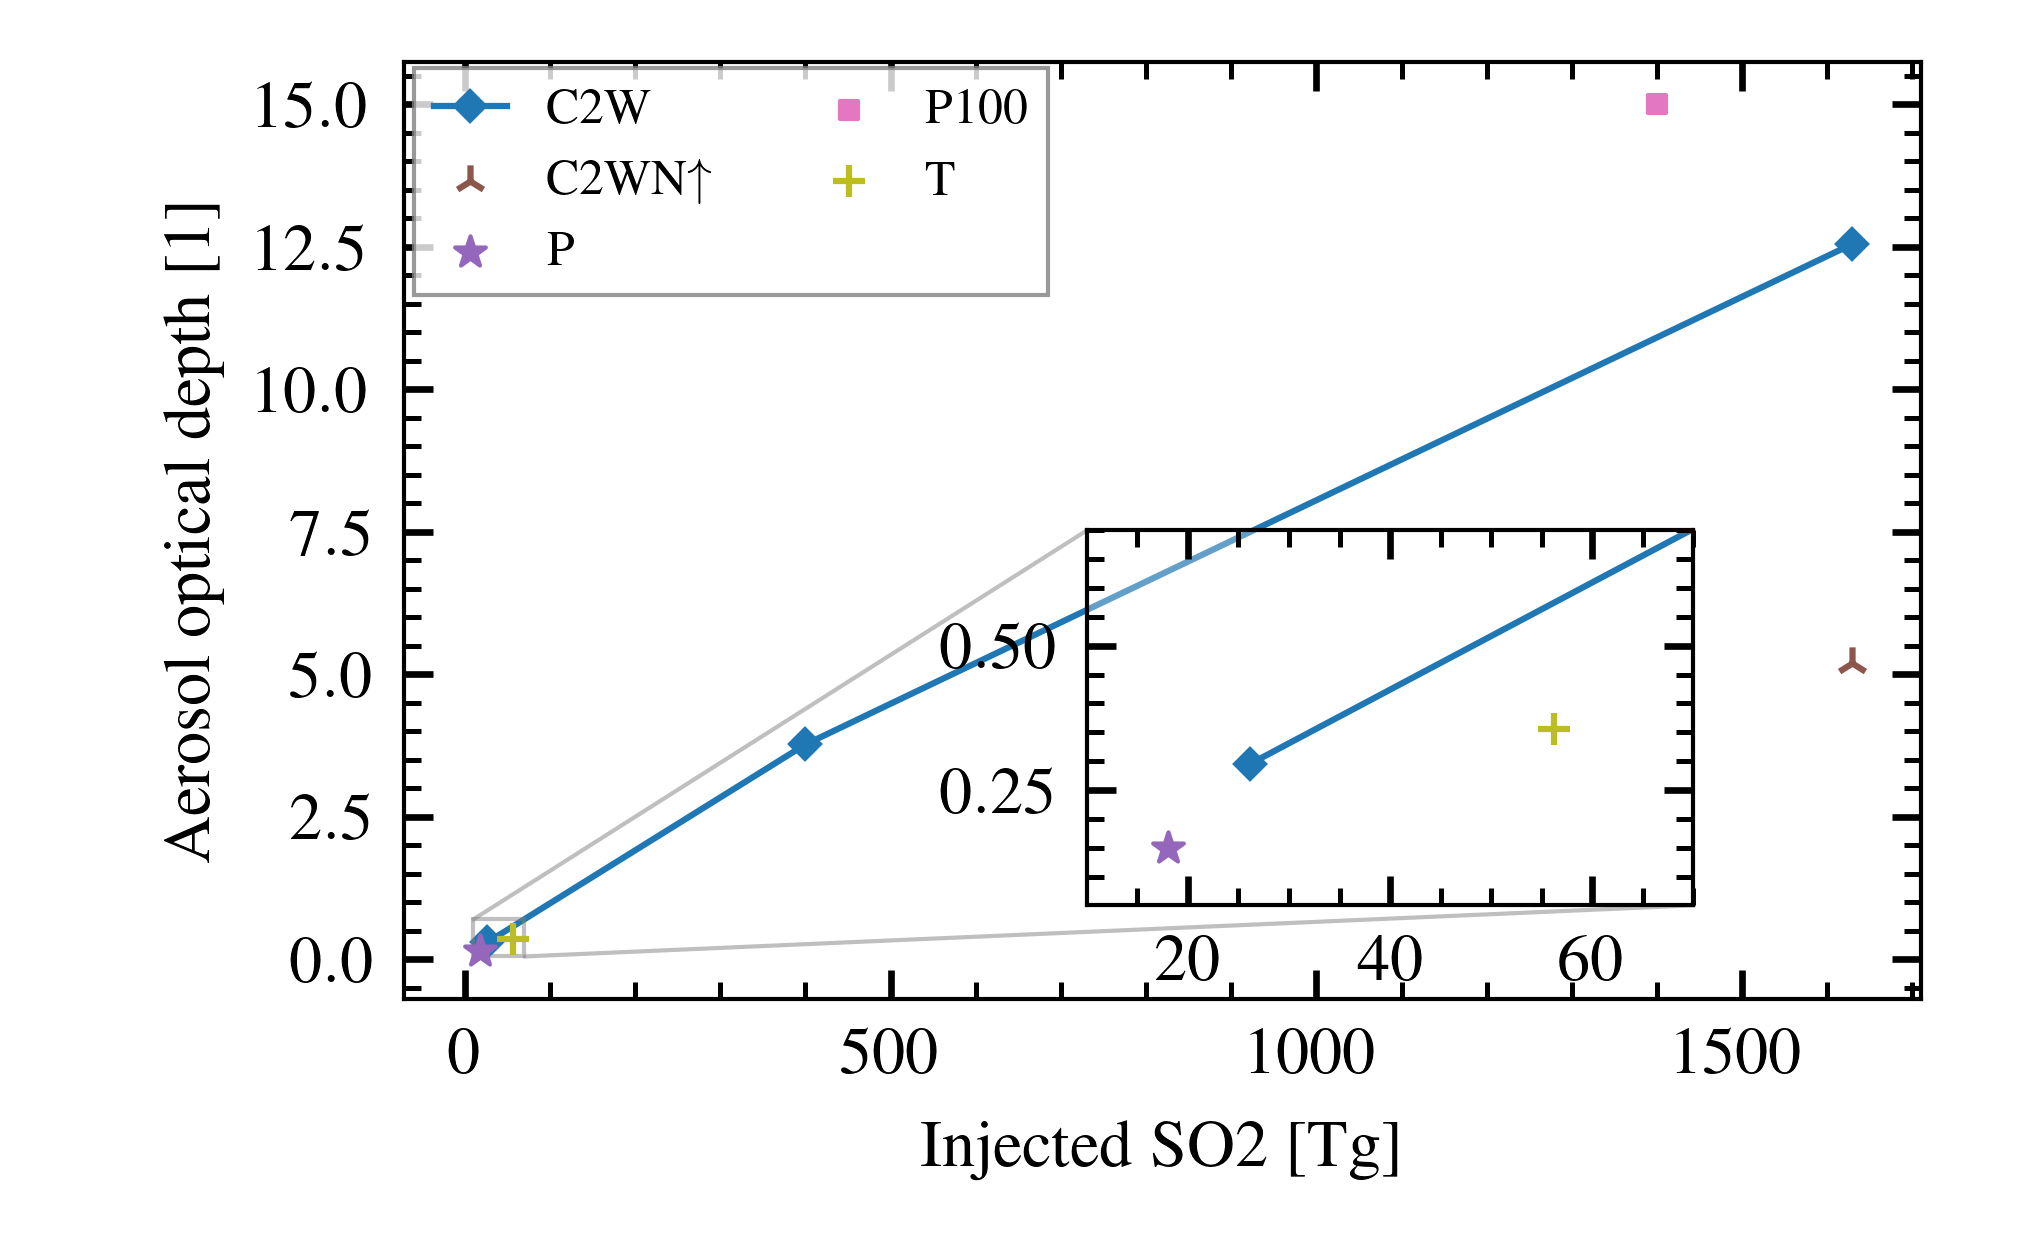
\includegraphics[width=0.95\linewidth]{figures/injection_vs_aod.png}
  \end{center}
  \caption{Injected \ce{SO2} versus \acrshort{aod}}%
  \label{fig:so2_vs_aod}
\end{figure}

With the almost linear relation between injected \ce{SO2} and \acrshort{aod}, we should
expect to see a similar plot for \iso{} versus \acrshort{rf} as for \acrshort{aod}
versus \acrshort{rf}. \iso[I] versus \acrshort{rf} is shown in \cref{fig:so2_vs_toa},
but where the absolute value of the \acrshort{rf} is potted along the \( y \)-axis. Just
as in \cref{fig:aod_vs_toa_full} we find the \acrshort{cesm2} data points to be heavily
damped in \acrshort{rf} compared to \iso. The same effect can be seen in the data from
\citet{ottobliesner2016} (labelled \textbf{C1C}, red points), but here the \acrshort{rf}
tend to bend off sooner, having a smaller \acrshort{rf} response to \iso{} than the
\acrshort{cesm2} data has. The simulations used by \citet{ottobliesner2016} was with
\acrshort{cesm} as well, but version 1 (\acrshort{cesm1}) and with a low-top atmosphere
(\acrshort{cam5}). The difference in model complexity might therefore be the reason why
the \iso{} give weaker \acrshort{rf} response for \citet{ottobliesner2016} than what we
find.

\begin{figure}[t]
  \begin{center}
    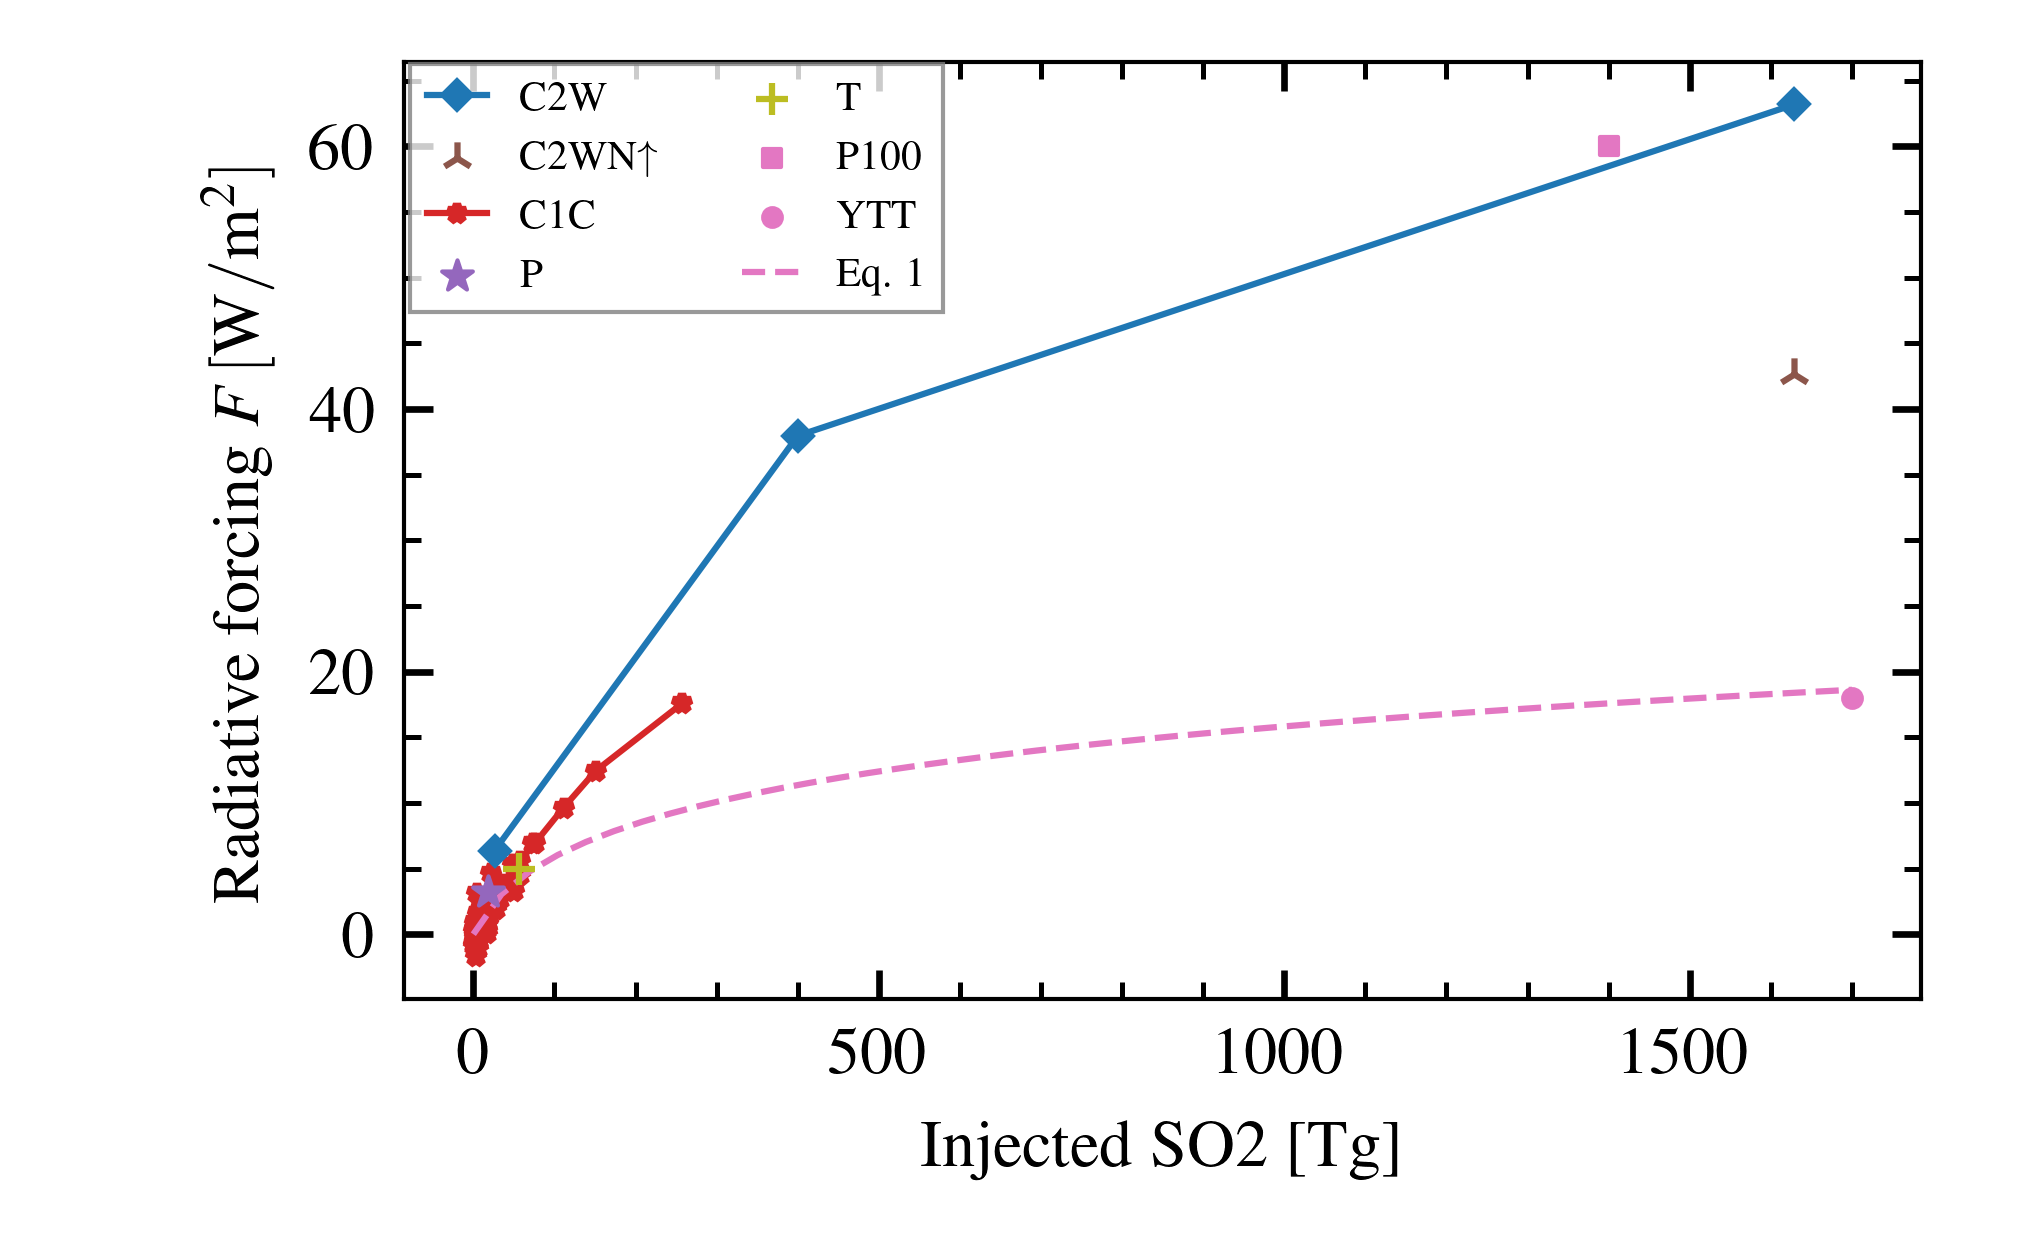
\includegraphics[width=0.95\linewidth]{figures/injection_vs_toa.png}
  \end{center}
  \caption{Injected \ce{SO2} versus \acrshort{rf} radiative imbalance}%
  \label{fig:so2_vs_toa}
\end{figure}

\Cref{fig:so2_vs_temp} show \iso{} versus temperature response. Just as in
\cref{fig:so2_vs_toa}, the data from the \acrshort{cesm2} simulations bend off, making
the temperature response less extreme for higher values of \iso. Again we see that the
data from the \acrshort{cesm1} simulations by \citet{ottobliesner2016} follow a
different path than the \acrshort{cesm2} data, with weaker temperature fluctuations for
a given \iso{}, as one would expect based on \cref{fig:so2_vs_toa}.

\begin{figure}[t]
  \begin{center}
    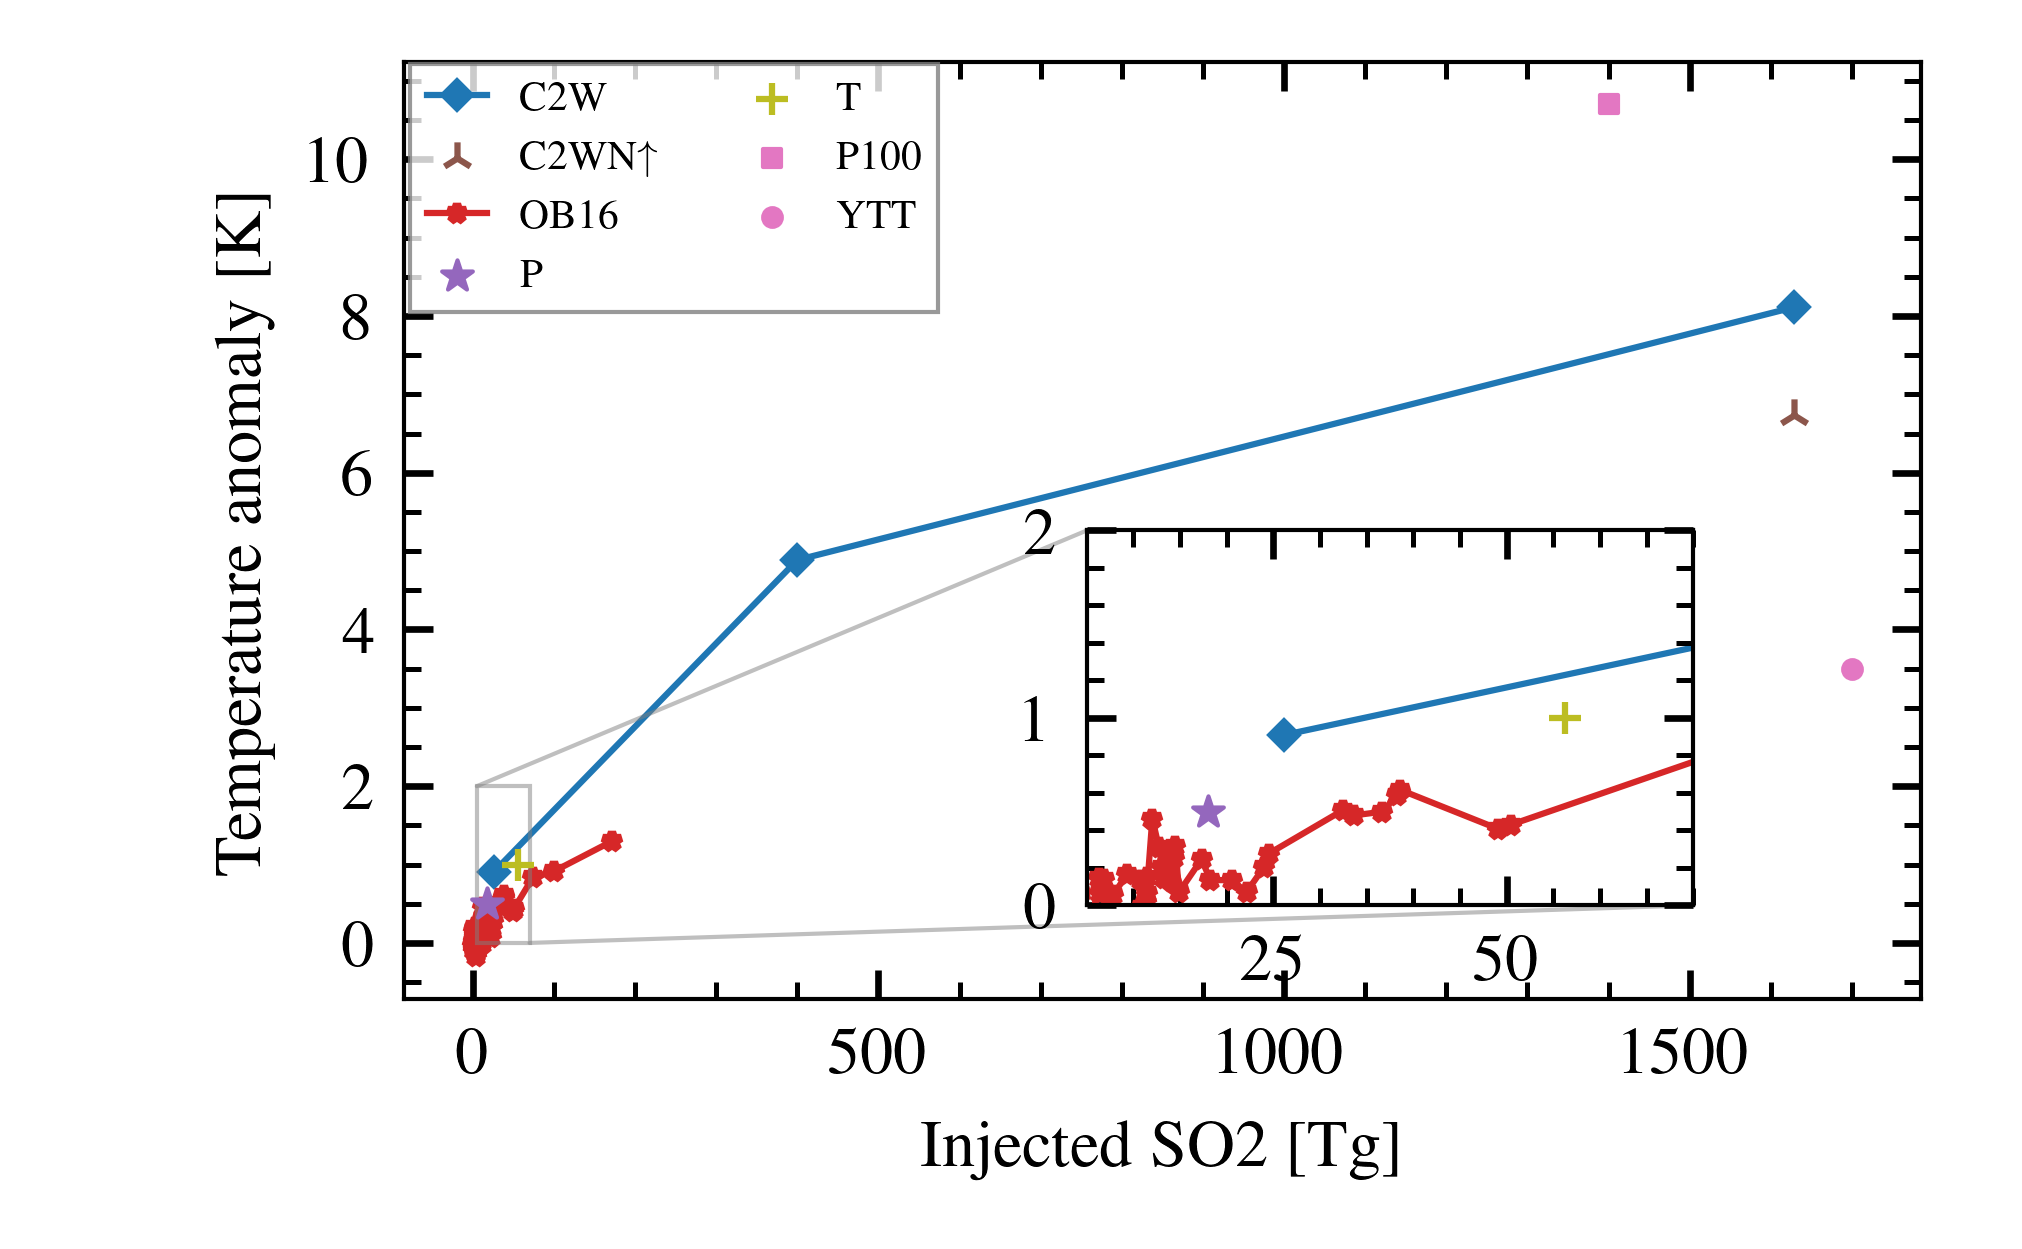
\includegraphics[width=0.95\linewidth]{figures/injection_vs_temperature.png}
  \end{center}
  \caption{Injected \ce{SO2} versus temperature}%
  \label{fig:so2_vs_temp}
\end{figure}

\Cref{fig:aod_vs_temp} should in the case of the \acrshort{cesm2} data points be very
similar in shape to the paths found in \cref{fig:so2_vs_temp} due to the close to linear
relationship found between \iso{} and \acrshort{aod} in \cref{fig:so2_vs_aod}. The
relationship between \acrshort{aod} and temperature is slightly more linear than what is
the case with \iso{} and temperature, but the tendency is still the same.

\begin{figure}[t]
  \centering
  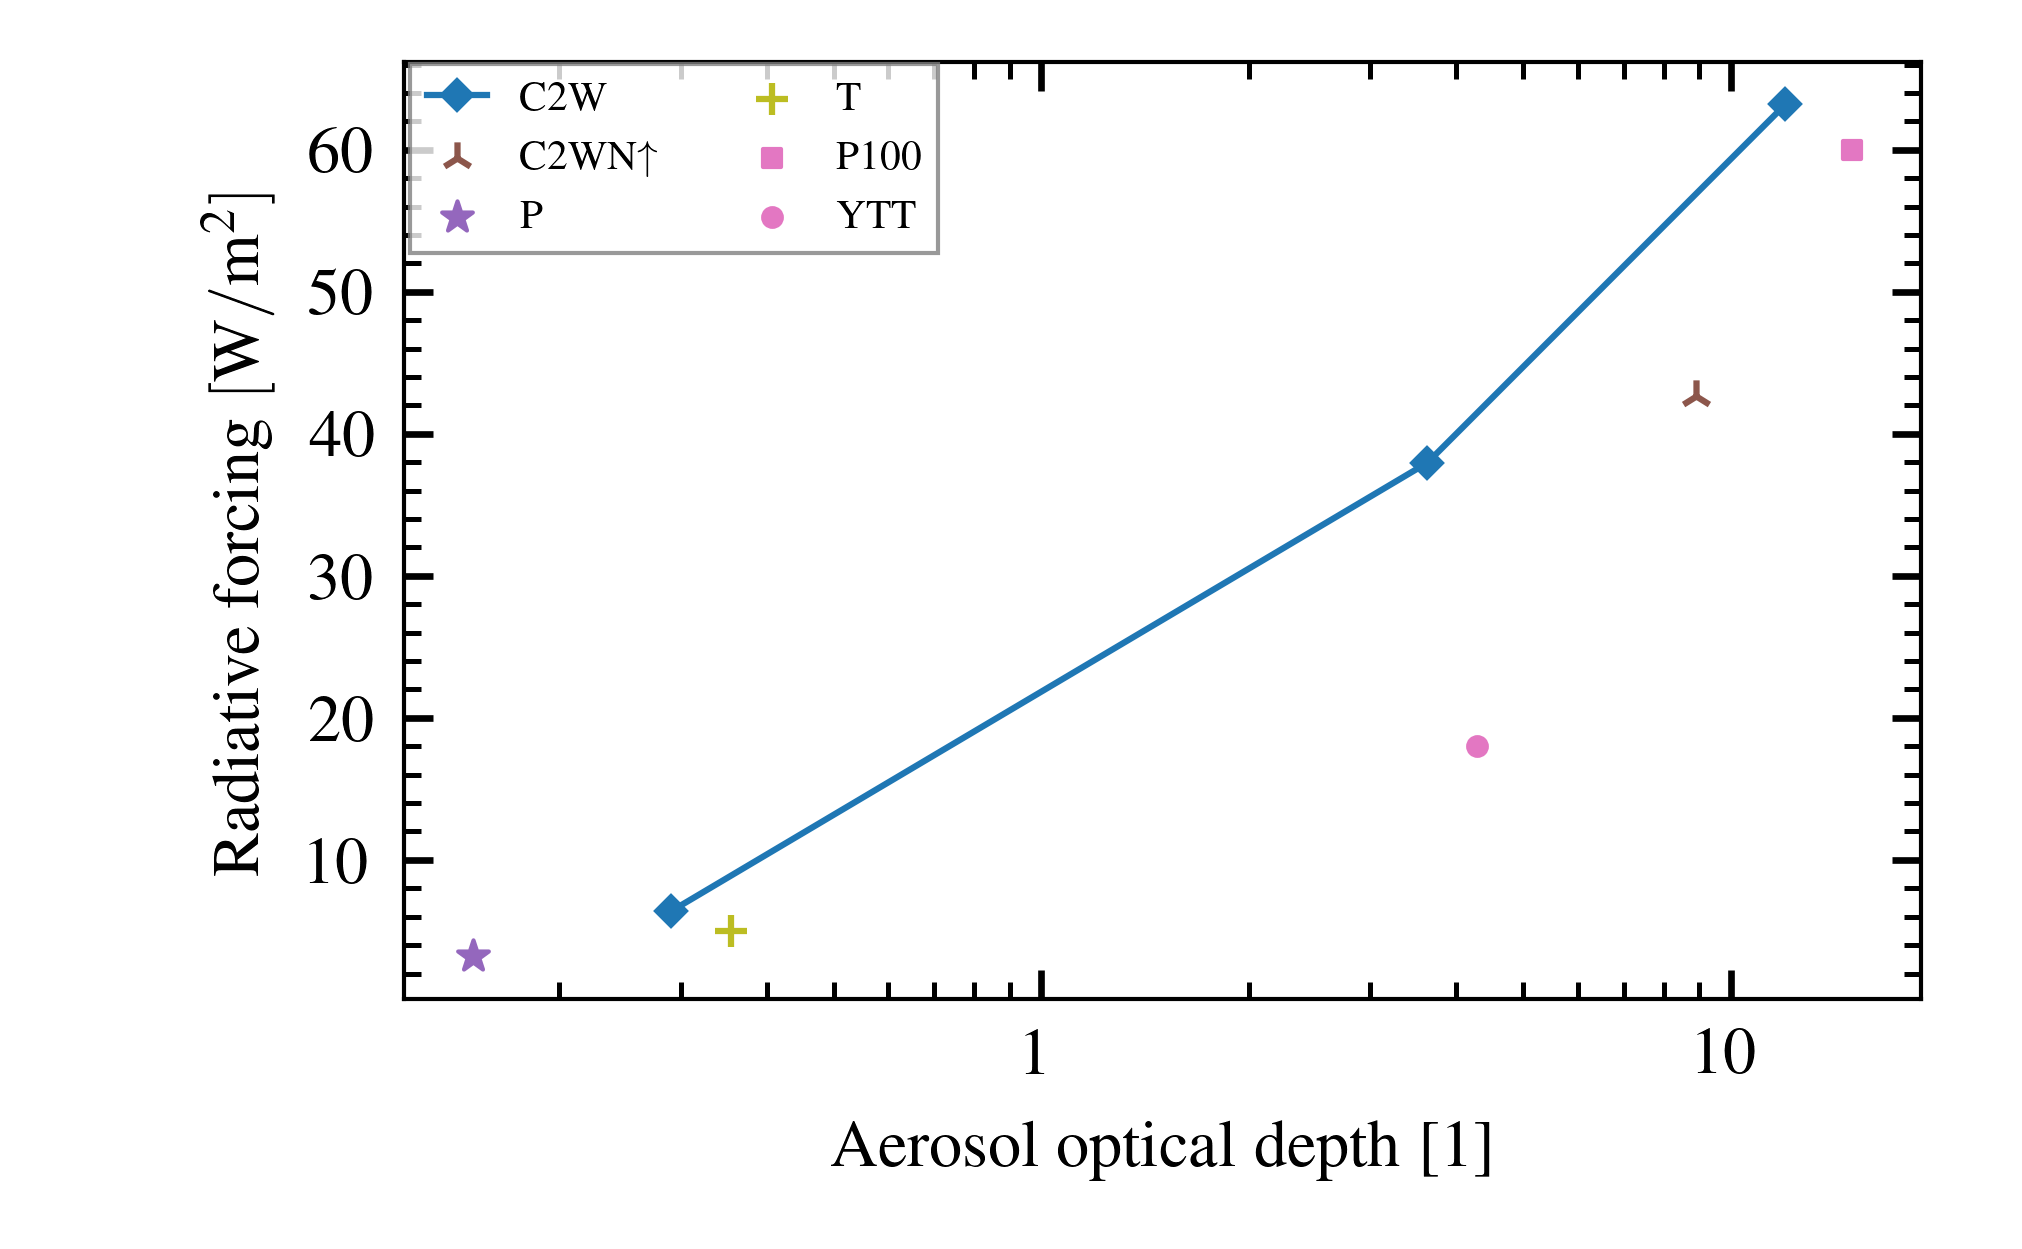
\includegraphics[width=0.95\linewidth]{figures/aod_vs_toa_logscale.png}
  \caption{\acrshort{aod} versus \acrshort{rf}}%
  \label{fig:aod_vs_toa_logscale}
\end{figure}

\begin{figure}[t]
  \begin{center}
    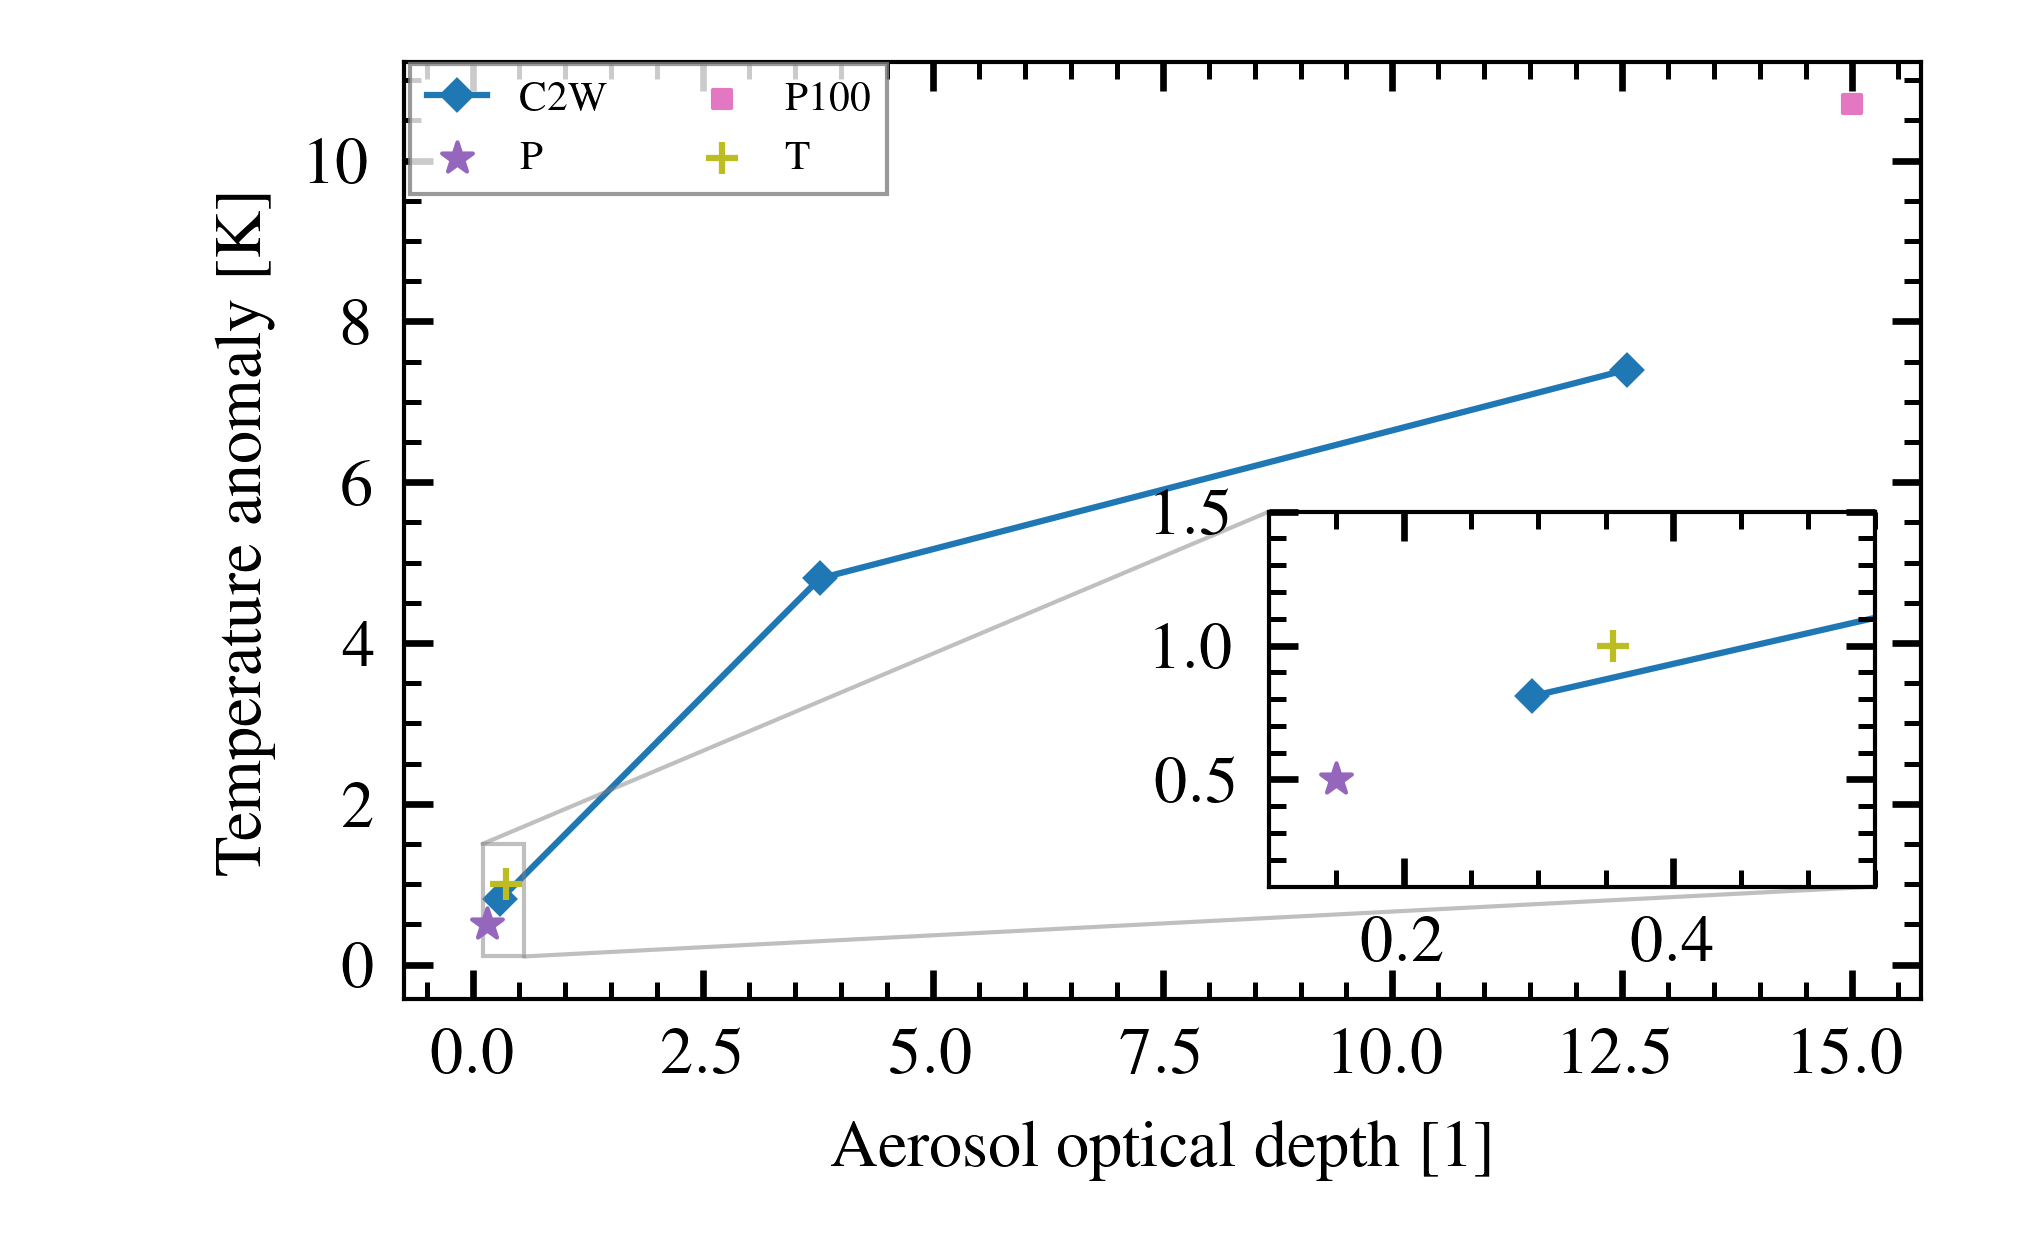
\includegraphics[width=0.95\linewidth]{figures/aod_vs_temperature.png}
  \end{center}
  \caption{\acrshort{aod} versus temperature}%
  \label{fig:aod_vs_temp}
\end{figure}

In \cref{fig:toa_vs_temp} we compare the \acrshort{rf} and temperature response. Both
the \acrshort{cesm2} data and the \acrshort{cesm1} from \citet{ottobliesner2016} show a
close to linear relationship between temperature and \acrshort{rf}, but where the
\acrshort{cesm2} data seem to lead to stronger temperature perturbations compared to
\acrshort{cesm1}. However, the overlap in data is not big, and the \acrshort{cesm2} data
is too sparse to make strong conclusions, in addition to the difference in model
complexity.

While the \acrshort{p100} data have been comparable to the strong \acrshort{cesm2} data
point in both \acrshort{aod} and \acrshort{rf}, the temperature response reported by
\citet{jones2005} is much stronger than what our strongest eruption caused. Since
\citet{jones2005} used the \acrshort{aod} forcing from Mt. Pinatubo multiplied by one
hundred, the shape during the whole phase could be significantly different to what a
super-eruption would create, even though the peak is representable, as we have seen in
\cref{fig:aod_arrays_normalized} where the \acrshort{aod} shape differ as the eruption
strength is increased. This might be enough to cause a much stronger temperature
perturbation.

\begin{figure}[t]
  \begin{center}
    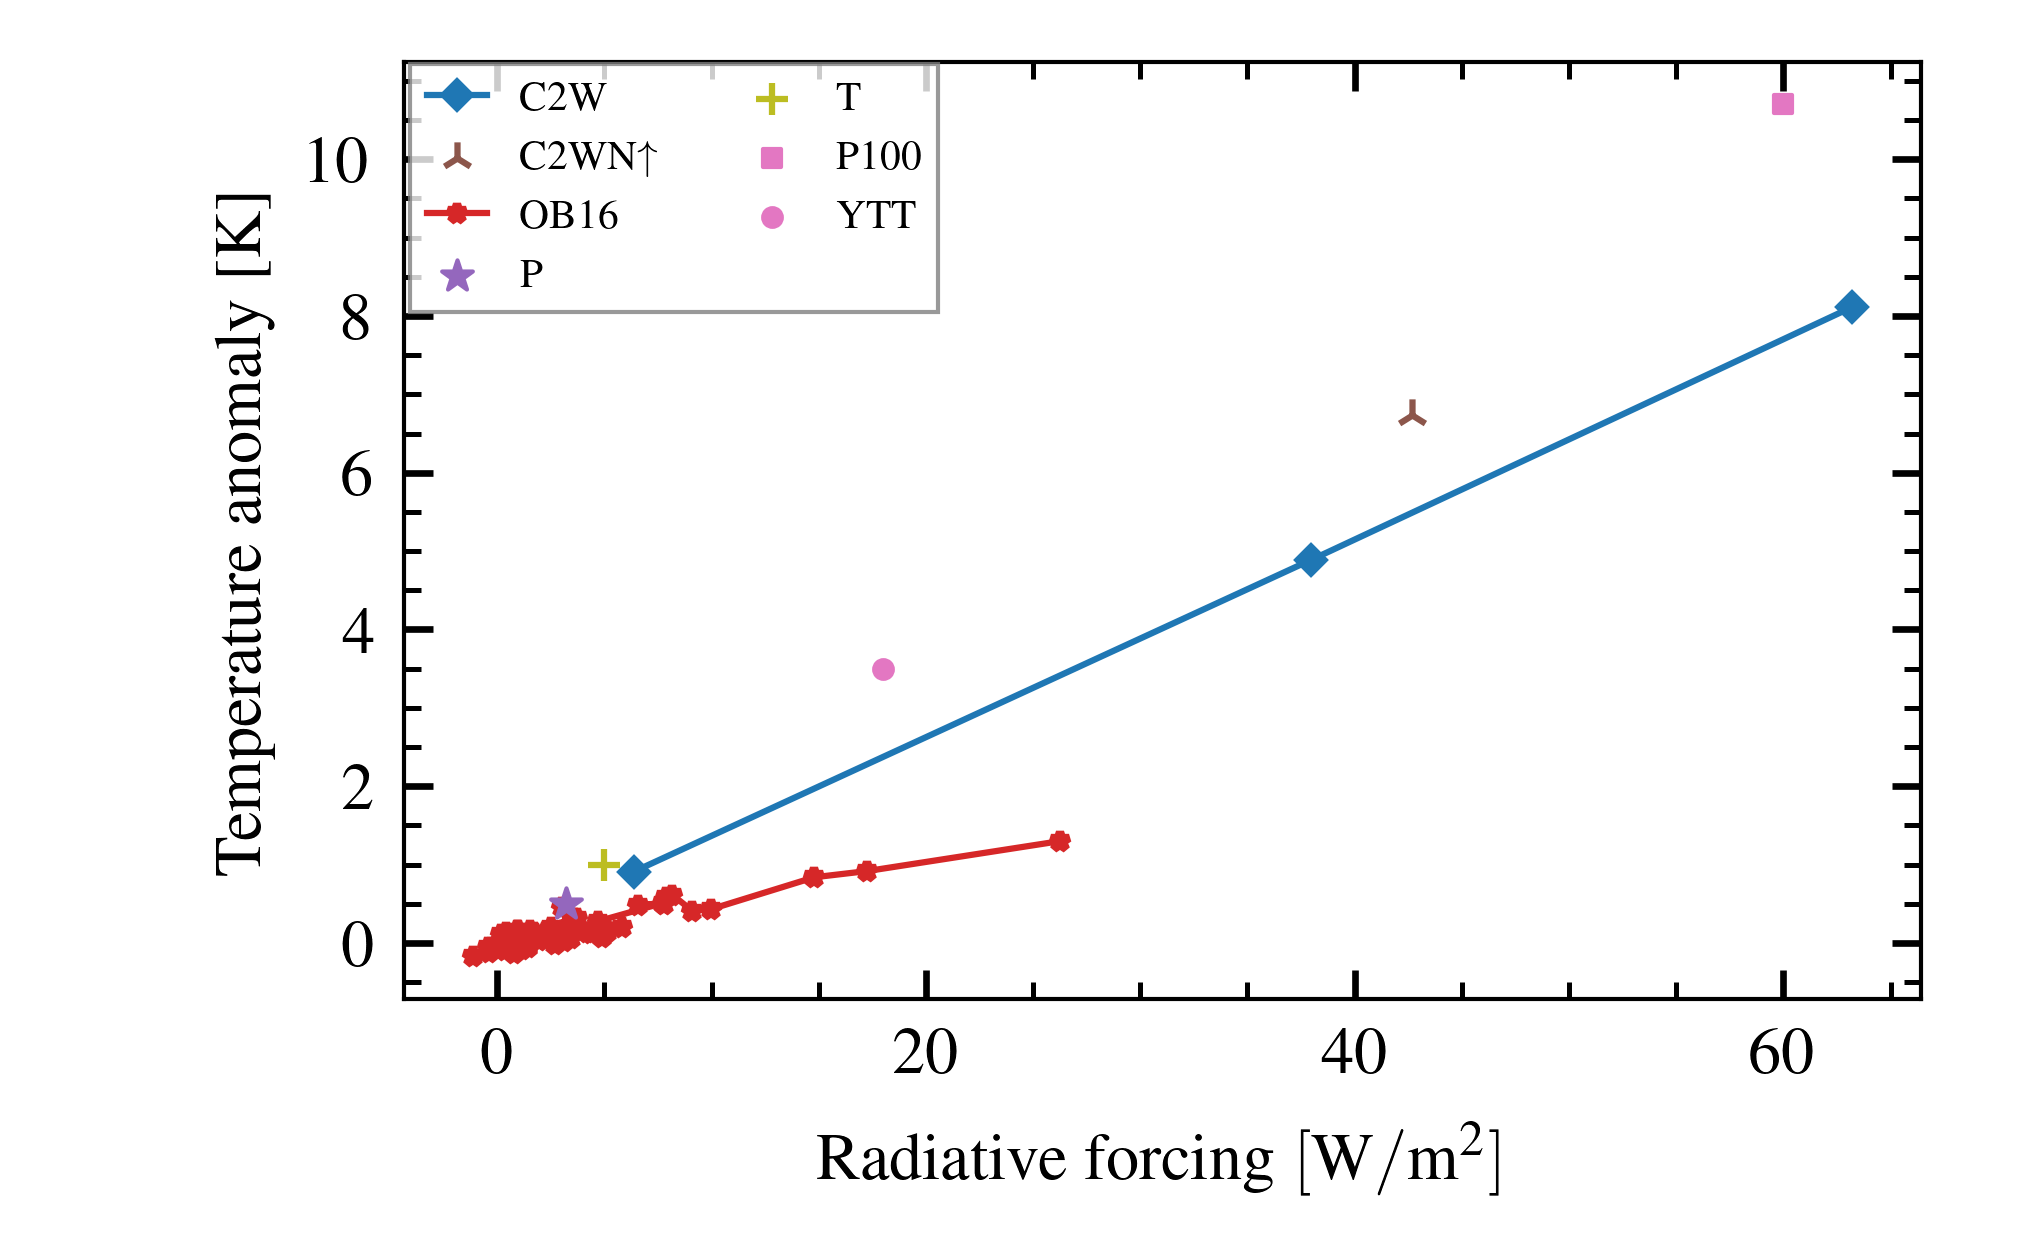
\includegraphics[width=0.95\linewidth]{figures/toa_vs_temperature.png}
  \end{center}
  \caption{\acrshort{rf} versus temperature}%
  \label{fig:toa_vs_temp}
\end{figure}

\section{Discussion \& Conclusions}

% NOTE: what we have done, future work, going back to points from introduction

In this paper we considered three large to super-volcano sized eruptions.

\clearpage

Todo:

\begin{itemize}
  \item Create an estimate of climate sensitivity from volcanoes
  \item Create plots also using the \(1-\mathrm{e}^{-\mathrm{SAOD}}\), like in Marshall et al.
        (2020)
\end{itemize}

\clearpage

% %%%%%%%%%%%%%%%%%%%%%%%%%%%%%%%%%%%%%%%%%%%%%%%%%%%%%%%%%%%%%%%%%%%%%%%%%%%%%%%%%%%%%%
% ACKNOWLEDGMENTS
% %%%%%%%%%%%%%%%%%%%%%%%%%%%%%%%%%%%%%%%%%%%%%%%%%%%%%%%%%%%%%%%%%%%%%%%%%%%%%%%%%%%%%%
% \acknowledgments

% Keep acknowledgments (note correct spelling: no ``e'' between the ``g'' and ``m'') as
% brief as possible. In general, acknowledge only direct help in writing or research.
% Financial support (e.g. grant numbers) for the work done, for an author, or for the
% laboratory where the work was performed is best acknowledged here rather than as
% footnotes to the title or to an author's name. Contribution numbers (if the work has
% been published by the author's institution or organization) should be included as
% footnotes on the title page, not in the acknowledgments.

% %%%%%%%%%%%%%%%%%%%%%%%%%%%%%%%%%%%%%%%%%%%%%%%%%%%%%%%%%%%%%%%%%%%%%%%%%%%%%%%%%%%%%%
% DATA AVAILABILITY STATEMENT
% %%%%%%%%%%%%%%%%%%%%%%%%%%%%%%%%%%%%%%%%%%%%%%%%%%%%%%%%%%%%%%%%%%%%%%%%%%%%%%%%%%%%%%
% \datastatement

% The data availability statement is where authors should describe how the data
% underlying the findings within the article can be accessed and reused. Authors should
% attempt to provide unrestricted access to all data and materials underlying reported
% findings. If data access is restricted, authors must mention this in the statement.

% %%%%%%%%%%%%%%%%%%%%%%%%%%%%%%%%%%%%%%%%%%%%%%%%%%%%%%%%%%%%%%%%%%%%%%%%%%%%%%%%%%%%%%
% APPENDIXES
% %%%%%%%%%%%%%%%%%%%%%%%%%%%%%%%%%%%%%%%%%%%%%%%%%%%%%%%%%%%%%%%%%%%%%%%%%%%%%%%%%%%%%%
%
% Use \appendix if there is only one appendix.
% \appendix

% Use \appendix[A], \appendix[B], if you have multiple appendixes.
% \appendix[A]

% Appendix title is necessary! For appendix title:
% \appendixtitle{}

% Appendix section numbering (note, skip \section and begin with \subsection)
% \subsection{First primary heading}

% \subsubsection{First secondary heading}

% \paragraph{First tertiary heading}

% Important!
% \appendcaption{<appendix letter and number>}{<caption>}
% must be used for figures and tables in appendixes, e.g.
%
% \begin{figure}
% \noindent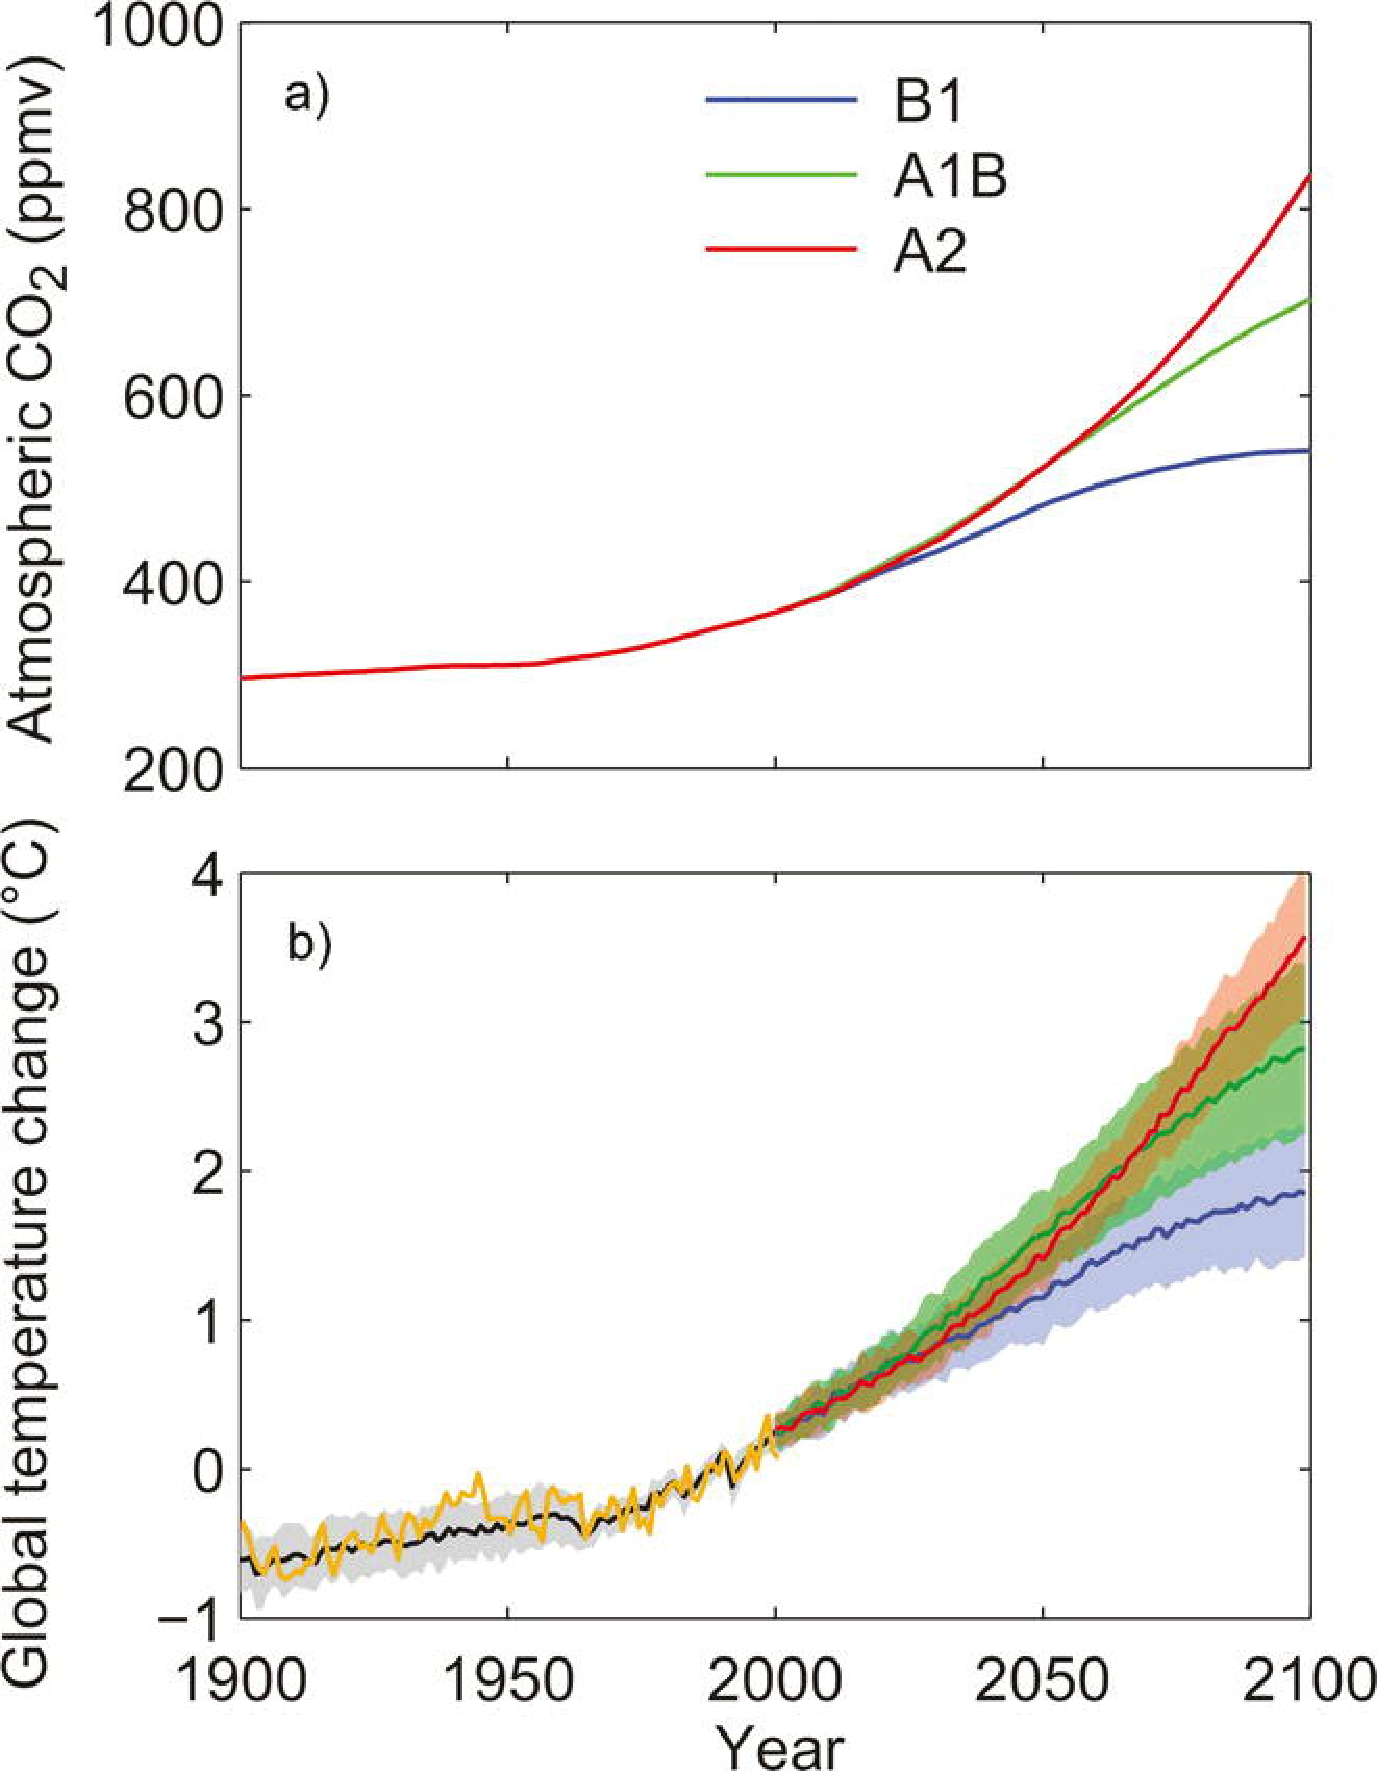
\includegraphics[width=19pc,angle=0]{figure01.pdf}\\
% \appendcaption{A1}{Caption here.}
% \end{figure}
%
% All appendix figures/tables should be placed in order AFTER the main figures/tables,
% i.e., tables, appendix tables, figures, appendix figures.
%
% %%%%%%%%%%%%%%%%%%%%%%%%%%%%%%%%%%%%%%%%%%%%%%%%%%%%%%%%%%%%%%%%%%%%%%%%%%%%%%%%%%%%%%
% REFERENCES
% %%%%%%%%%%%%%%%%%%%%%%%%%%%%%%%%%%%%%%%%%%%%%%%%%%%%%%%%%%%%%%%%%%%%%%%%%%%%%%%%%%%%%%
% Make your BibTeX bibliography by using these commands:
\bibliographystyle{ametsoc2014}
\bibliography{references}
\clearpage
\printglossary[type=\acronymtype,title=List of Acronyms]
% %%%%%%%%%%%%%%%%%%%%%%%%%%%%%%%%%%%%%%%%%%%%%%%%%%%%%%%%%%%%%%%%%%%%%%%%%%%%%%%%%%%%%%
% TABLES
% %%%%%%%%%%%%%%%%%%%%%%%%%%%%%%%%%%%%%%%%%%%%%%%%%%%%%%%%%%%%%%%%%%%%%%%%%%%%%%%%%%%%%%
% Enter tables at the end of the document, before figures.
%
% \begin{table}[t]
%   \caption{This is a sample table caption and table layout.  Enter as many tables as
%     necessary at the end of your manuscript. Table from Lorenz (1963).}\label{t1}
%   \begin{center}
%     \begin{tabular}{ccccrrcrc}
%       \hline\hline
%       $N$  & $X$  & $Y$  & $Z$  \\
%       \hline
%       0000 & 0000 & 0010 & 0000 \\
%       0005 & 0004 & 0012 & 0000 \\
%       0010 & 0009 & 0020 & 0000 \\
%       0015 & 0016 & 0036 & 0002 \\
%       0020 & 0030 & 0066 & 0007 \\
%       0025 & 0054 & 0115 & 0024 \\
%       \hline
%     \end{tabular}
%   \end{center}
% \end{table}

% %%%%%%%%%%%%%%%%%%%%%%%%%%%%%%%%%%%%%%%%%%%%%%%%%%%%%%%%%%%%%%%%%%%%%%%%%%%%%%%%%%%%%%
% FIGURES
% %%%%%%%%%%%%%%%%%%%%%%%%%%%%%%%%%%%%%%%%%%%%%%%%%%%%%%%%%%%%%%%%%%%%%%%%%%%%%%%%%%%%%%
% Enter figures at the end of the document, after tables.
%
% \begin{figure}[t]
%   \noindent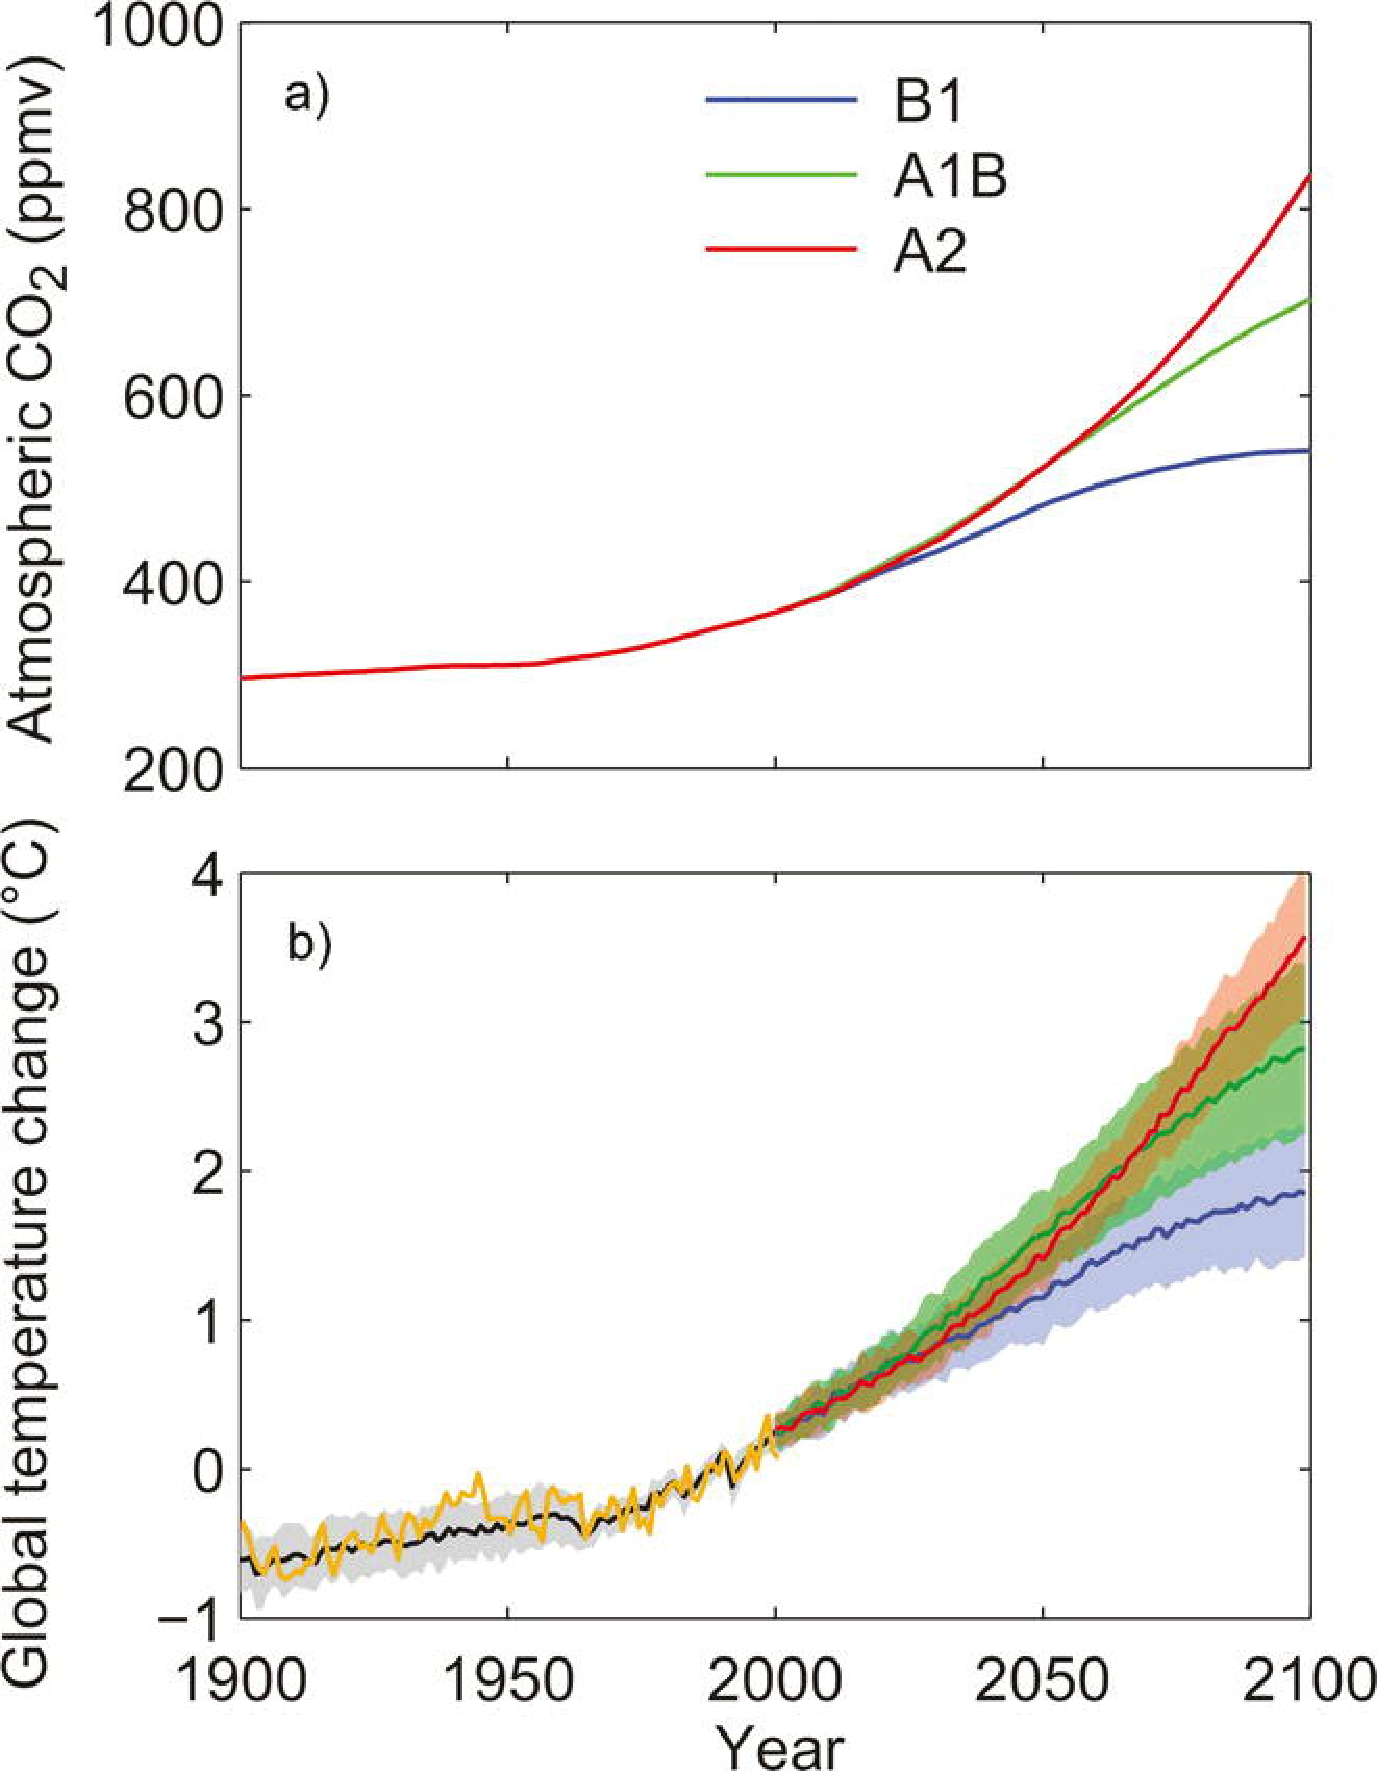
\includegraphics[width=19pc,angle=0]{figure01.pdf}\\
%   \caption{Enter the caption for your figure here.  Repeat as
%     necessary for each of your figures. Figure from \protect\cite{Knutti2008}.}\label{f1}
% \end{figure}

\end{document}
